\documentclass{article}
\usepackage[T1]{fontenc}
\usepackage[utf8]{inputenc}
\usepackage{geometry}
\geometry{a4paper, textwidth=5.8in, textheight=9in}
\usepackage[export]{adjustbox}
\usepackage[final]{pdfpages}
\usepackage{graphicx}
\usepackage{float}
\usepackage{subcaption}
\usepackage{tabularx}
\usepackage{xltabular}
\usepackage{makecell}
\usepackage[numbers]{natbib}
\usepackage{placeins}
\PassOptionsToPackage{hyphens}{url}
\usepackage[colorlinks=true,linkcolor=blue,citecolor=red,urlcolor=blue]{hyperref}
\usepackage{doi}
\graphicspath{{./Figures/}}

%% Helper macros
\newcommand{\inlinepath}[1]{`\path{#1}'}
\newcommand{\hwport}[1]{\texttt{\detokenize{#1}}}
\newcommand{\parameter}[1]{\textit{\detokenize{#1}}}
\newcommand{\module}[1]{\textit{\detokenize{#1}}}
\newcommand{\command}[1]{\texttt{\detokenize{#1}}}
\newcommand{\configvalue}[1]{params.\textit{\detokenize{#1}}}

%% FAQ style
\newcounter{troublecnt}[subsection]
%\renewcommand*\thetroublecnt{\arabic{section}.\arabic{troublecnt}}
\renewcommand*\thetroublecnt{Issue \arabic{troublecnt}}
\makeatletter
\newcommand\trouble{\@ifstar\troublenotnumbered\troublenumbered}
\makeatother
\newcommand{\troublenumbered}[1]{%
    \refstepcounter{troublecnt}%
    %{\it \makebox[1cm][l]{\textbf{\thetroublecnt}} #1}
    \begin{samepage}%
        \begin{description}%
            \item[\textbf{\thetroublecnt}] {\it #1}%
        \end{description}%
    \end{samepage}\nopagebreak[4]%
}
\newcommand{\troublenotnumbered}[1]{%
    \refstepcounter{troublecnt}%
    {\it #1}%
}

% Relax some LaTeX defaults for better treatment of figures:
    % See p.105 of "TeX Unbound" for suggested values.
    % See pp. 199-200 of Lamport's "LaTeX" book for details.
    %   General parameters, for ALL pages:
    \renewcommand{\topfraction}{0.95}  % max fraction of floats at top
    \renewcommand{\bottomfraction}{0.9} % max fraction of floats at bottom
    %   Parameters for TEXT pages (not float pages):
    \setcounter{topnumber}{2}
    \setcounter{bottomnumber}{2}
    \setcounter{totalnumber}{4}     % 2 may work better
    \setcounter{dbltopnumber}{2}    % for 2-column pages
    \renewcommand{\dbltopfraction}{0.9} % fit big float above 2-col. text
    \renewcommand{\textfraction}{0.07}  % allow minimal text w. figs
    %   Parameters for FLOAT pages (not text pages):
    \renewcommand{\floatpagefraction}{0.7}  % require fuller float pages
    % N.B.: floatpagefraction MUST be less than topfraction !!
    \renewcommand{\dblfloatpagefraction}{0.7} % require fuller float pages

  % remember to use [htp] or [htpb] for placement

% Code listings
\usepackage{listings}
\usepackage{lstautogobble}
\lstset{language=[LaTeX]Tex,%C++,
  morekeywords={PassOptionsToPackage,selectlanguage},
  keywordstyle=\color{blue},%\bfseries,
  basicstyle=\small\ttfamily,
  %identifierstyle=\color{NavyBlue},
  commentstyle=\color{gray}\ttfamily,
  stringstyle=\rmfamily,
  numbers=none,%left,%
  numberstyle=\scriptsize,%\tiny
  numberbychapter=true,
  stepnumber=5,
  numbersep=8pt,
  showstringspaces=false,
  breaklines=true,
  %frameround=ftff,
  %frame=single,
  belowcaptionskip=.75\baselineskip,
  %frame=L,
  autogobble=true,
  mathescape=true,
  frame=l,
  xleftmargin=.04\textwidth,
  float=htp,
}
% Language Extensions
\lstdefinestyle{Verilog}{language=Verilog,
  morekeywords={assert, assume, property},
}

% Tabular helper
\newcommand{\vcenterothercols}[1]{\noindent\parbox[c]{\hsize}{
    \vspace{.25\baselineskip}
    #1
    \vspace{.25\baselineskip}
    }}
\newcolumntype{R}{>{\raggedright\arraybackslash}X}

% Really long URLs
\urldef{\VTRdocRRG}\url{https://docs.verilogtorouting.org/en/latest/vpr/file_formats/#routing-resource-graph-file-format-xml}


\begin{document}

\title{ZUMA User's Manual}
\author{Tobias Wiersema, Arne Bockhorn, Alexander D. Brant,\\ Monica Keerthipati, Nithin S. Sabu, and Felix P. Jentzsch}
\date{30.05.2020}
\maketitle
\tableofcontents

%\clearpage
\section{Introduction}
This repository contains the ZUMA FPGA overlay architecture system that was introduced by
\begin{NoHyper}\citeauthor{brantlemieux2012ZUMA} in \citeyear{brantlemieux2012ZUMA}\end{NoHyper}~\cite{brantlemieux2012ZUMA,brant2013MT} and later extended by Wiersema, Bockhorn and Platzner~\cite{wiersemaBP2014ZUMAReconOS,wiersemaBP2016ZUMAReconOS} and several students of Paderborn University.
ZUMA is an open-source, cross-compatible embedded FPGA architecture that is intended as an overlay on top of an existing FPGA, in essence an ``FPGA-on-an-FPGA.''
This approach of a virtual FPGA has a number of benefits, including bitstream compatibility between different vendors and parts, compatibility with open FPGA tool flows, and the ability to embed some programmable logic into systems on FPGAs without the need for releasing or recompiling the master netlist.

%\clearpage
This manual provides an overview of the ZUMA system and contains the following elements:
\begin{enumerate}
    \item Instructions on how to prepare the repository  and external tools to be able to run the overlay generation flow (Section~\ref{sec:installation}).
    \item Instructions on how to get started with the basic tool flow of ZUMA (Section~\ref{sec:gettingstarted}).
    \item Instructions for including a generated overlay into a new or existing FPGA design (Section~\ref{sec:include_ZUMA_in_project}).
    \item Details on advanced usage scenarios, an in-depth description of the underlying FPGA model of the virtual FPGA and how it corresponds to the build parameters of the ZUMA system, as well as an overview of the generated output files and their layout (Section~\ref{sec:advancedusage}).
    This should allow you to generate advanced, custom-built virtual FPGAs that exactly fit to your needs.
\end{enumerate}

\noindent The folders included in this repository contain a number of components needed to use ZUMA, as well as examples and tests.
The directory structure is as follows:\\[1.5mm]
\renewcommand{\arraystretch}{1.4}%
\begin{tabularx}{\textwidth}{lX}
    \hline
    doc/               &  Contains this documentation.  \\
    example/           &  Contains a ZUMA preferences file, sample Verilog and timing SDF files, and a script to compile.  \\
    external/          &  Required third party tools as GIT submodules. \\
    misc/              &  Contains a patch that is required to use (the very old) VPR6 with ZUMA. \\
    source/            &  Scripts to generate the ZUMA Verilog components and bitstreams. \\
    tests/             &  Included scripts used to test ZUMA components. \\
    tests/integration/ &  Python unit tests to automatically assert the correct installation and behavior of the ZUMA scripts. \\
    verilog/           &  Verilog files used for building a ZUMA system, included platform specific and simulation files. \\
    license.txt        &  The license under which ZUMA can be used. \\
    Makefile           &  Global Makefile to prepare a working tool flow for overlay generation. \\
    toolpaths.py       &  Global path setup to tie in the third party tools -- can be adapted if the provided tool submodules shall not be used. \\
    \hline \\
\end{tabularx}

\clearpage
\subsection{Contributors and Brief History}
Many wonderful people have contributed to the ZUMA project. This section is a (very) brief history of how the project was shaped by them.

In \textbf{2012}, Alexander D. Brant wrote the first version of the ZUMA generator scripts as a graduate student under the guidance of Guy G. F. Lemieux, with whom he published the first paper on ZUMA~\cite{brantlemieux2012ZUMA}.

In \textbf{2013\,/\,2014}, Tobias Wiersema, as a research assistant to Marco Platzner, extended the implementation to also support sequential circuits, by extending the eLUT LUTRAM macro instantiation, added the optional permutation layer to the overlay, and embedded it into a ReconOS\footnote{\url{http://www.reconos.de}} hardware thread that can receive its configuration at runtime from a software thread through shared memory. Although this embedding is not bundled here, it was the basis for streamlining the configuration process within the test bench wrapper.

In the years \textbf{2014 -- 2016}, Arne Bockhorn rewrote much of the ZUMA code as a student research assistant to Tobias Wiersema, and extended it with the timing analysis features, realized the initial description of the Clos network-based IIBs, made it compatible to VTR1\,/\,VPR7, wrote the Bitstream-to-BLIF back-translation tool, and helped with the ReconOS integration.
In this period, Arne, Marco, and Tobias also published their two ZUMA papers~\cite{wiersemaBP2014ZUMAReconOS,wiersemaBP2016ZUMAReconOS}.

In \textbf{2017\,/\,2018}, Nithin S. Sabu and Monica Keerthipati realized the first Xilinx Vivado version of ZUMA as graduate students together with their student project group ReCoTroy, supervised by Tobias Wiersema. They also contributed the corresponding guide in Section~\ref{sec:include_ZUMA_in_Xilinx_project}.

In \textbf{2019}, Felix P. Jentzsch implemented the first Xilinx Vivado nested block design that contained a ZUMA overlay as a student research assistant to Tobias Wiersema. He contributed the corresponding instructions in Section~\ref{ssub:ZUMA_in_xilinx_troubleshooting}.

In \textbf{2020}, Arne Bockhorn rewrote the generator scripts again to make it more maintainable and compatible to version 8 of VTR\,/\,VPR, extended the timing analysis to a full virtual timing-driven placement \& routing flow version, enabled a ZUMA overlay description in hierarchical HDL, and wrote integration tests to be able to ensure the correctness of features and to spot regressions.
Tobias Wiersema aggregated all available ZUMA documentation and compiled the first versions of this user's manual, and enabled the integration of the external tools directly within the context of this GIT repository.
Arne's and Tobias' goal was to provide the most modern, compatible, feature complete, and comprehensively documented ZUMA version to render its usage and adoption for future projects as easy as possible.







\clearpage
\section{Installation}
\label{sec:installation}
ZUMA scripts are written in Python, and require a valid Python install to run.
The scripts are tested with Python 2.7.
You will also need the python libraries plumbum and numpy and optional graphviz.
To just get started, just run
\begin{verbatim}
make
\end{verbatim}
This will fetch and build all required tools and run a unit test that asserts the correct behavior of the tool chain. If this finishes with an \emph{OK}, then your ZUMA copy is ready to be used, and you can skip the rest of this section.
If you run into build errors, please refer to the failing tool's GitHub site for help.

\subsection{VTR flow}
The VTR\footnote{\url{https://verilogtorouting.org/}} tool set must also be installed in order to compile with ZUMA.
ZUMA does not call the VTR flow directly, but tools thereof and requires files that are generated by them.

For convenience, a GIT submodule is located under \inlinepath{external/vtr} that points to a VTR version of the official VTR GitHub repository\footnote{\url{https://github.com/verilog-to-routing/vtr-verilog-to-routing}} that is known to work with this ZUMA version.
This included VTR version can be build by just issuing a standard \command{make} in ZUMA's top directory, or in the \inlinepath{external} subdirectory.

Should you want to use an existing VTR installation with theses scripts, you can adapt the variable VTR\_DIR that is used in scripts to find the VTR install.
To change it globally, update the file \inlinepath{toolpaths.py} in the base directory to point to your installation location.

VPR versions prior to 7 (which are thus very old by now) do not automatically dump the routing resource graph and lack a command line switch to do so.
Since this file is needed by ZUMA, you need to activate the dumping of this file via a debug switch at compile time.
For modern versions of VTR and VPR, you will not need to perform the following steps and can skip to the next section.

For VPR 6 a patch file is located in the directory \inlinepath{$VTR_DIR/vpr/SRC/route/}, which can be applied to the file \inlinepath{rr_graph.c}
, by calling:
\begin{verbatim}
cat (ZUMA dir)/misc/patch.txt (VTR dir)/vpr/SRC/route/rr_graph.c > \
    (VTR dir)/vpr/SRC/route/rr_graph.c'
\end{verbatim}
The patch instructs VPR to always dump its routing graph to the file \inlinepath{rr_graph.echo}.
If using a different version, defining CREATE\_ECHO\_FILES in \inlinepath{rr_graph.c} will enable this functionality.

\subsection{Yosys}
\label{sub:Yosys}
To enable an automatic verification of the functional equivalence between the generated overlay configuration and the original HDL specification, you additionally need Yosys\footnote{\url{http://www.clifford.at/yosys/}}.

For convenience, a GIT submodule is located under \inlinepath{external/yosys} that points to a Yosys version of the official Yosys GitHub repository\footnote{\url{https://github.com/YosysHQ/yosys}} that is known to work with this ZUMA version.
This included Yosys version can be build by just issuing a standard \command{make} in ZUMA's top directory, or in the \inlinepath{external} subdirectory.

Should you want to use an existing Yosys installation with theses scripts, you can adapt the variable yosysDir that is used in scripts to find the Yosys install.
To change it globally, update the file \inlinepath{toolpaths.py} in the base directory to point to your installation location.












\clearpage
\section{Getting started}%
\label{sec:gettingstarted}
\subsection{Running the Example}
Calling the Python script
\begin{verbatim}
compile.sh test.v
\end{verbatim}
will automatically build the ZUMA system Verilog \inlinepath{ZUMA_custom_generated.v},
and a bitstream hex file \inlinepath{output.hex}, which can be used to synthesize and configure a ZUMA system.
By passing other circuit files, modifying the example ZUMA configuration file \inlinepath{zuma_config.py}, or providing an alternative configuration file via the \emph{-{}-config} command line switch, custom architectures and bitstreams can be generated.



\subsection{ZUMA Tool Flow}
An overview of the flow of tools required to generate ZUMA overlays, and configurations for them, is depicted in Figure~\ref{fig:zumaflow}, adapted from~\cite{wiersemaBP2016ZUMAReconOS}.

It roughly works as follows:
Starting with the ZUMA parameters in the \inlinepath{zuma_config.py} the \command{compile.sh} uses the templates stored in \inlinepath{source/templates/} to generate the architecture description of the overlay in VTR's XML format.
Leveraging this architecture description and the virtual circuit, e.g., \inlinepath{test.v}, the VTR flow (or more specifically ODIN II, ABC, and VPR) can deduce the complete routing resources of the overlay, which are saved into a file (custom format in VTR \(\leq\) 7 and XML in VTR 8), and can also synthesize, place and route the virtual circuit to the described architecture, resulting in descriptive files for the netlist, the placement and the routing.
The ZUMA scripts take all of these generated files and compute the correct configuration for each programmable entity of the overlay, i.e., eLUTs and programmable interconnect points, and save the complete virtual configuration as ZUMA bitstream into the files \inlinepath{output.hex} and \inlinepath{output.hex.mif}.
While the former is the correct bitstream version as defined for ZUMA, the latter is an undecorated collection of only the configuration bits and nothing more, ready-to-use for inclusion by vendor tools as memory content.
For a more in-depth, step-by-step discussion of the flow, and for using advanced features such as static timing analysis or timing-driven placement and routing of virtual circuits, see Section~\ref{sub:zuma_flow_details}.

\begin{figure}[htp]
    \centering
    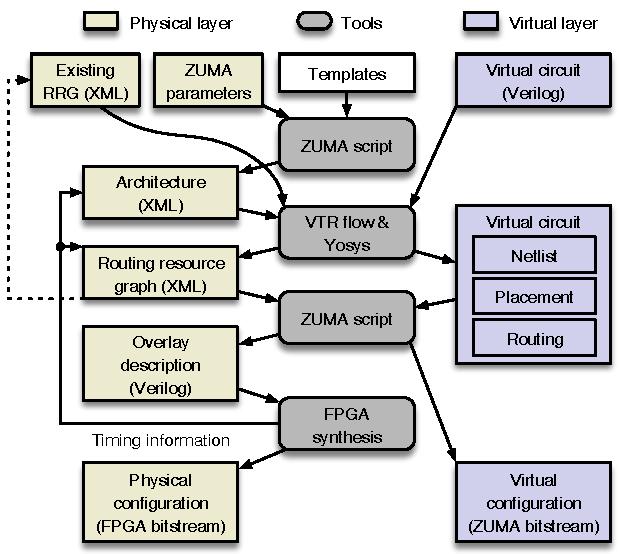
\includegraphics[width=0.7\textwidth]{Figures/zumaflow}%
    \caption{The tool flow to generate overlays and configurations.}
    \label{fig:zumaflow}
\end{figure}

For the physical side of things, the ZUMA scripts generate a description of the complete overlay fabric in Verilog, \inlinepath{ZUMA_custom_generated.v}, using LUTRAM instantiation macros to define all programmable entities.
This Verilog file can be included into a regular FPGA project to actually synthesize an overlay onto a physical device.
For more details of this inclusion, see Section~\ref{sec:include_ZUMA_in_project}.




\subsection{Bit to BLIF}
You can also reverse ZUMA's virtual synthesis and (re-)build a BLIF file from the generated bitstream. To this end, you can call the script
\begin{verbatim}
>example/extract_logic_function.sh output.hex.mif output.blif HasClock HasReset
\end{verbatim}
where \inlinepath{output.hex.mif} is the bitstream you want to build your BLIF from,
\inlinepath{output.blif} the name of the BLIF file you want to create and \parameter{HasClock} and \parameter{HasReset} are two booleans [True/False] which indicate if the circuit uses a clock and\,/\,or a reset signal.
Those two signal properties cannot be read from the bitstream so you have to specify them.

Additionally the script requires the same \inlinepath{zuma_config.py} architecture parameter configuration that was used to build the \inlinepath{output.hex.mif} initially, because the architecture details can also not be read from the bitstream.













\section{Caveats and Restrictions}
A constraint for the virtual circuit file is that the head of the model must have the following signature:
\begin{verbatim}
verilog-module-name ([clock], reset, [input-name-1, input-name-2 , ... ])
\end{verbatim}
The clock and reset signal must have the given names and positions for the scripts to recognize their special behavior.
The reset is treated as the first input on the FPGA.
The declaration of a clock is optional.

The LUTRAMs used in the ZUMA architecture and contained in this repository are generated using Xilinx and Altera macros. To use a different LUTRAM or memory, instantiate it in the file \inlinepath{lut_custom.v}, and define a new platform (e.g., PLATFORM\_STRATIXIV) in the file \inlinepath{define.v} to select this LUTRAM.

Note that the Altera macros have not been maintained and that for the current ZUMA version thus only the Xilinx side is tested and guaranteed to work with current vendor tool flows.
Especially support for sequential virtual circuits has so far only been implemented for Xilinx projects.














\clearpage
\section{Including a ZUMA Overlay in a Project}
\label{sec:include_ZUMA_in_project}

Once the Verilog architecture is created, and a hex bitstream is generated, the ZUMA system can be compiled and used.
The generated Verilog file that describes the virtual fabric, along with the files in the \inlinepath{verilog/generic/} and \inlinepath{verilog/platform/(platform)/} directories should be included in a new Xilinx / Altera project, although getting it to work for Altera devices might require some (read: significant amount of) additional work.
We will describe the intent and general process here, for specific details on how to include it in a Xilinx Vivado project, please refer to Section~\ref{sec:include_ZUMA_in_Xilinx_project}.

The generated hex file should be placed in the project directory, and specified as the initial contents of the ZUMA configuration memory.
The top level file \inlinepath{ZUMA_TB_wrapper} includes a memory block which references the hex file \inlinepath{output.hex} that should be generated by the ZUMA tools and included with the project.
Note that sequential circuits are so far only supported in Xilinx projects.

If you change the configuration memory size, or the configuration width, you have to create an appropriate new memory using the vendor tools.
Runtime configuration of the ZUMA overlay is performed by loading each block of memory in the hex file to the port \hwport{config_data}, along with its address to \hwport{config_addr}, and asserting the corresponding \hwport{config_en} port.
Configuration completes when all data are loaded.

The ports \hwport{fpga_inputs} and \hwport{fpga_outputs} provide the interface between the physical and virtual FPGA logic.
As described in the original ZUMA paper~\cite{brantlemieux2012ZUMA} and Brant's master's thesis~\cite{brant2013MT}, the pins are located at the edges of the array, begin at the grid coordinate (0,1), and increase in the Y direction first.
The pins can be fixed to correspond to those of the input Verilog by specifying a pin location file when running VPR placement.

If you want to use the timing analysis or want to build a BLIF from a hex file,
see the timing and bit to BLIF readme files.

\clearpage
\subsection{Including a ZUMA Overlay in a Xilinx Vivado Project}
\label{sec:include_ZUMA_in_Xilinx_project}
For the inclusion of a generated ZUMA overlay into a Xilinx Vivado project, we provide a more detailed explanation here along with screenshots.
When following these steps, you should be able to synthesize a working, configurable ZUMA overlay with your project.

\begin{enumerate}

    \item Create a new project in Vivado by including the source files in the following directories:
    \begin{itemize}
        \item \path{verilog/generic}
        \item \path{verilog/platforms/xilinx}
    \end{itemize}
    Do not copy the files into the project, as they will be common to all projects. %Refer figure \ref{fig:addfiles}.

    %\begin{figure}[H]
    %\centering
    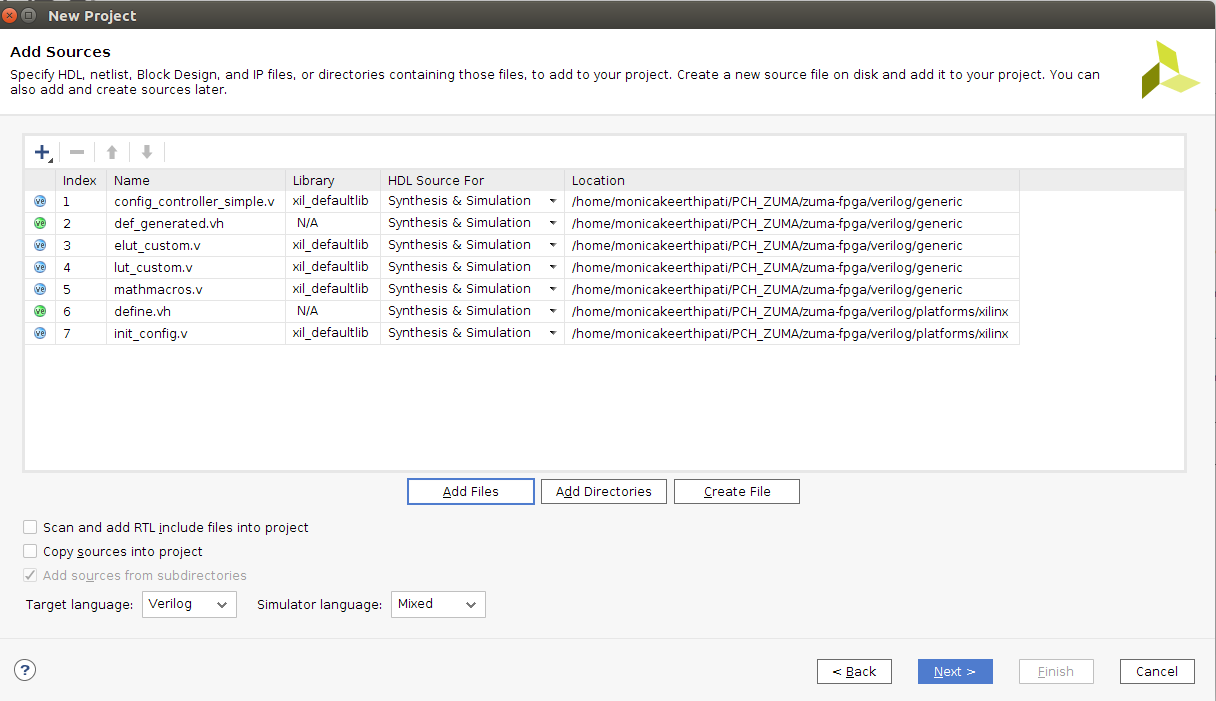
\includegraphics[width=.95\linewidth]{Figures/addfiles.png}
    %\label{fig:addfiles}
    %\end{figure}

    You might want to copy the file \inlinepath{verilog/generic/ZUMA_TB_wrapper.v} to the Vivado project, however, since this will be the top test bench for the project we are building here, so you might want to adapt this.

    %\begin{figure}[H]
    %\centering
    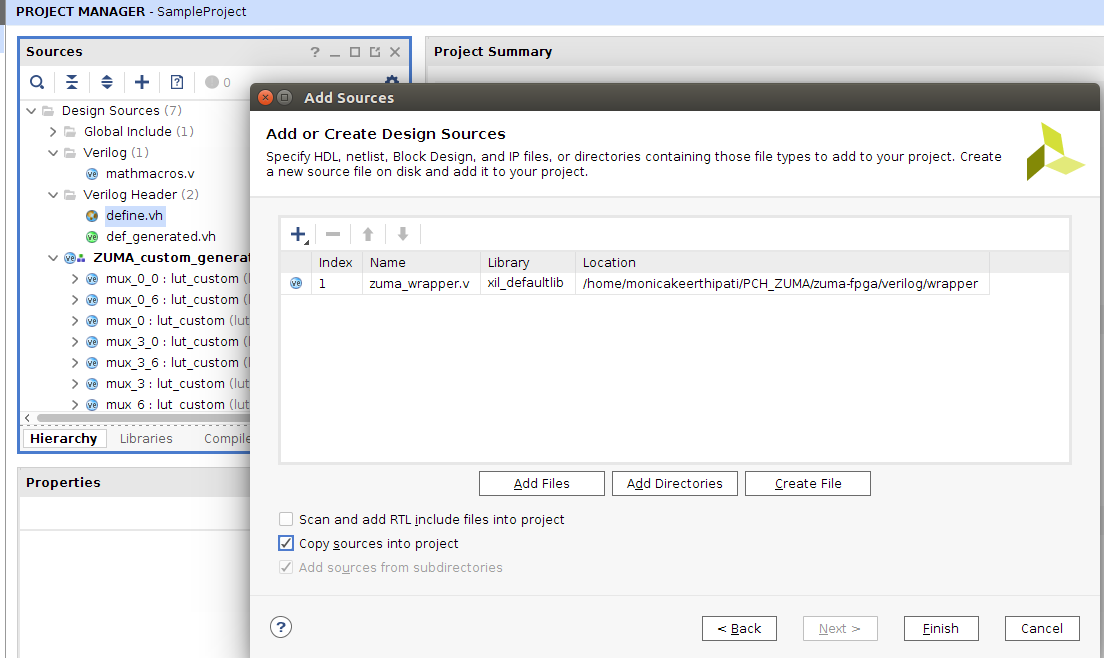
\includegraphics[width=0.95\linewidth]{Figures/vivado6.png}
    %\label{fig:vivado6}
    %\end{figure}

    \clearpage
    \item Click on \emph{Add sources} and add the following source files also to the project: %Refer figure \ref{fig:vivado5}.
    \begin{itemize}
        \item \path{example/ZUMA_custom_generated.v} -- overlay description
        \item \path{example/output.hex.mif} -- virtual configuration
        \item \path{example/def_generated.vh} -- generated header file
    \end{itemize}
    This time, you can choose whether or not to check \emph{Copy sources into project}. While these files change for each project, and thus could be copied, not copying them will force Vivado to read them from the ZUMA directory, so that when you regenerate them, they should be included in the new version.
    Should you, however, generate overlays for multiple projects in your ZUMA directory, it would be safer to copy them into the Vivado project.

    %\begin{figure}[H]
    %\centering
    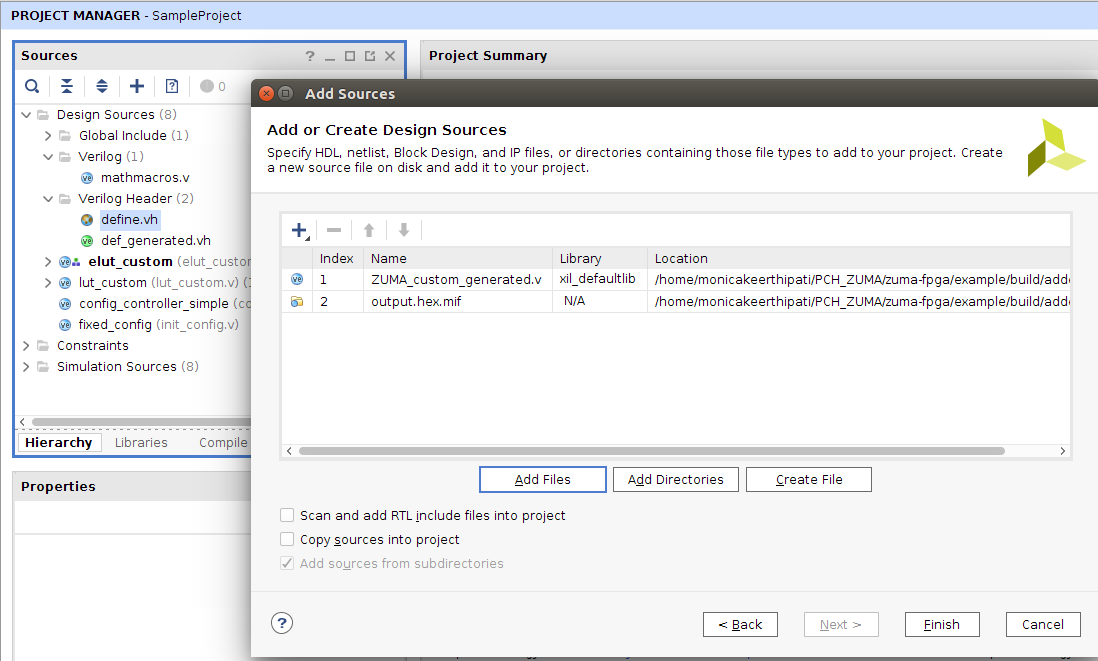
\includegraphics[width=0.95\linewidth]{Figures/vivado5.png}
    %\label{fig:vivado5}
    %\end{figure}

    %\clearpage
    \item Right click on \inlinepath{define.vh} and click \emph{Set Global Include} as shown. \\
    Do the same for \inlinepath{def_generated.vh}.%in figure \ref{fig:globalinclude}.

    %\begin{figure}[H]
    %\centering
    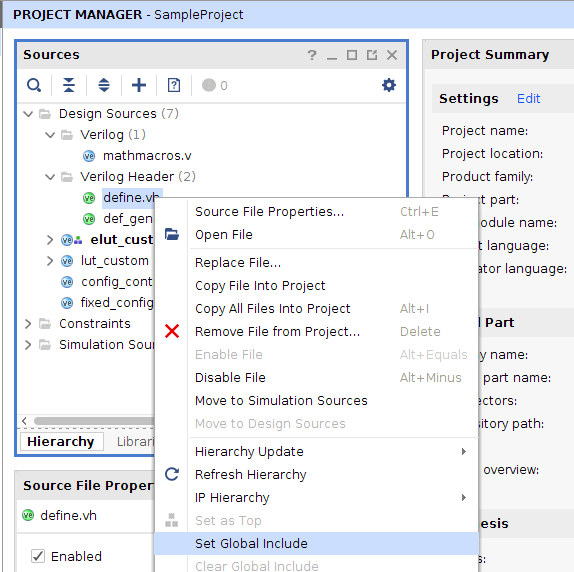
\includegraphics[width=0.5\linewidth]{Figures/globalinclude.png}
    %\label{fig:globalinclude}
    %\end{figure}

    \clearpage
    \item From the IP catalog, select the \emph{Distributed Memory Generator} core as shown. % in \ref{fig:vivado10}.
    Change the component name to \hwport{lut_xilinx}. Set \emph{Data Width} to 1. Change \emph{Memory Type} to \emph{Simple Dual Port RAM} and click \emph{OK}. %Refer figure \ref{fig:vivado11} for this step.
    This will include the basic building block of ZUMA into the project -- the LUTRAMs -- which the overlay will instantiate a hundredfold.

    %\begin{figure}[H]
    %\centering
    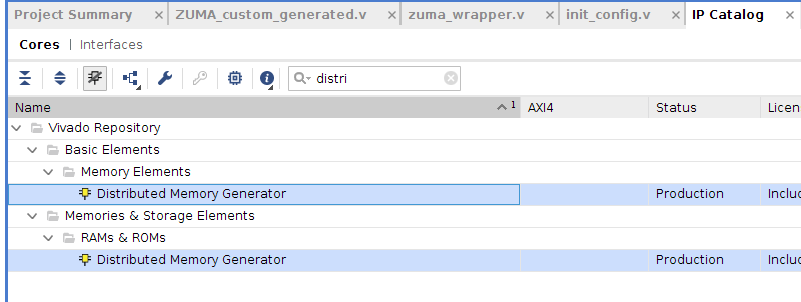
\includegraphics[width=0.7\linewidth]{Figures/vivado10.png}
    %\label{fig:vivado10}
    %\end{figure}

    %\begin{figure}[H]
    %\centering
    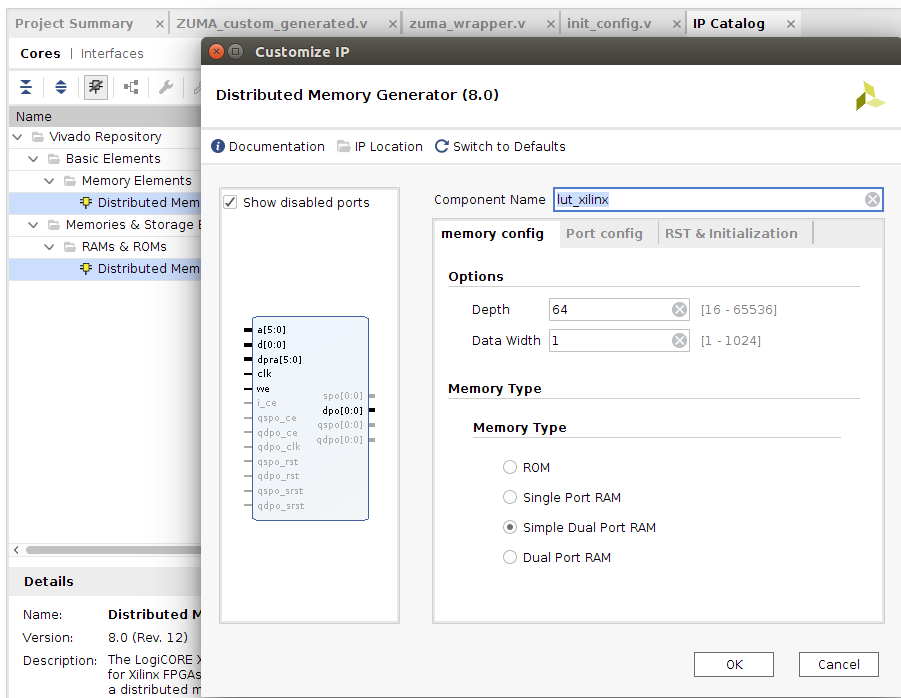
\includegraphics[width=0.7\linewidth]{Figures/vivado11.png}
    %\label{fig:vivado11}
    %\end{figure}

    \clearpage
    \item In the \emph{Generate Output Products} window that appears, set Synthesis Options to \emph{Out of context per IP} and click \emph{Generate}. %Refer figure \ref{fig:vivado12}.

    %\begin{figure}[H]
    %\centering
    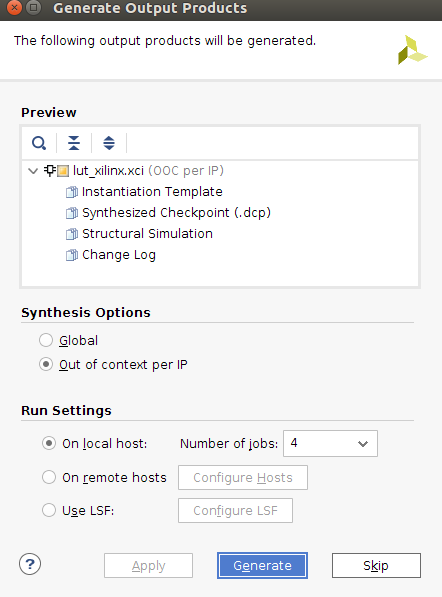
\includegraphics[width=0.5\linewidth]{Figures/vivado12.png}
    %\label{fig:vivado12}
    %\end{figure}

    \item Since the implementation of virtual sequential circuits, ZUMA requires a special version of this building block for its eLUTs. Hence, add the \emph{Distributed Memory Generator} core a second time now, but this time with different settings. Change the component name to \hwport{elut_xilinx}. Set \emph{Data Width} again to 1, and change \emph{Memory Type} also to \emph{Simple Dual Port RAM}. Do NOT dismiss the dialog, but proceed to the next tab now.

    %\begin{figure}[H]
    %\centering
    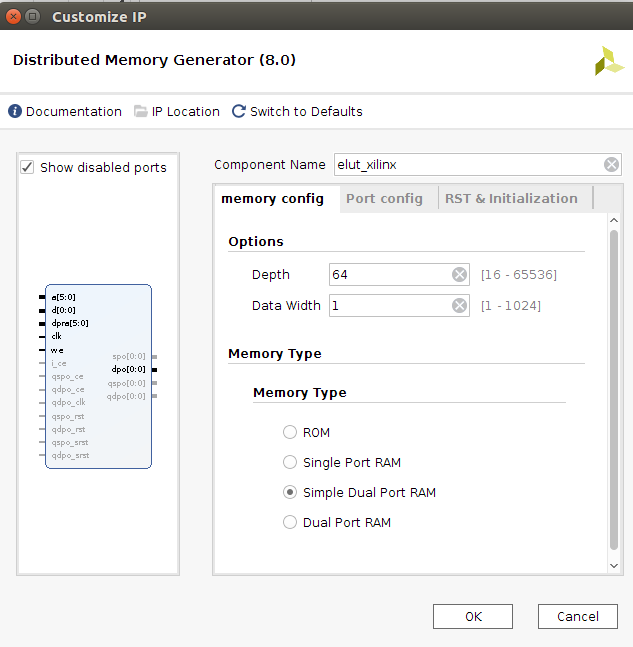
\includegraphics[width=0.7\linewidth]{Figures/vivado13.png}
    %\label{fig:vivado13}
    %\end{figure}

    In the \emph{Port config} tab, set \emph{Output Options} to \emph{Both}. Proceed to the final tab.

    %\begin{figure}[H]
    %\centering
    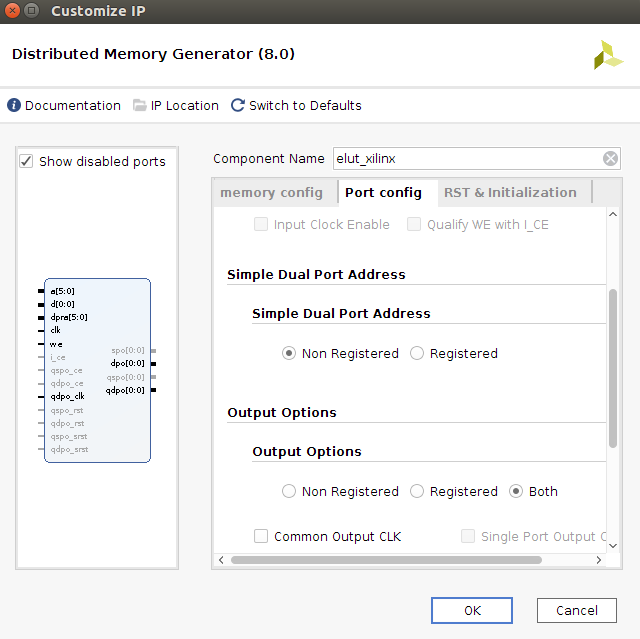
\includegraphics[width=0.7\linewidth]{Figures/vivado14.png}
    %\label{fig:vivado14}
    %\end{figure}

    In the \emph{RST and Initialization} tab, check \emph{Reset QSDPO} in \emph{Reset Options}.

    %\begin{figure}[H]
    %\centering
    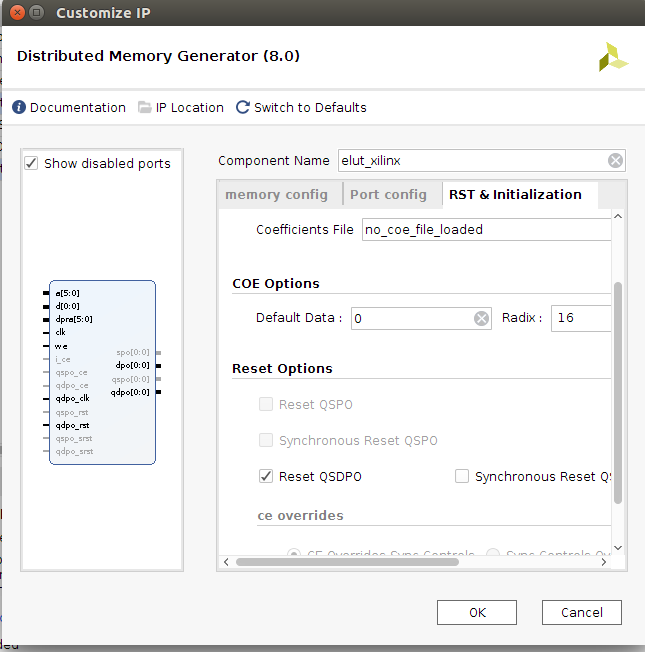
\includegraphics[width=0.7\linewidth]{Figures/vivado15.png}
    %\label{fig:vivado15}
    %\end{figure}

    Now you can finally click \emph{OK} and in the next window (\emph{Generate Output Products}) click \emph{Generate} again with \emph{Out of context per IP} settings. %The figures \ref{fig:vivado13}, \ref{fig:vivado14} and \ref{fig:vivado15} represent this step in a detailed manner.

    \clearpage
    \item Modify the \inlinepath{ZUMA_TB_wrapper.v} file based on your needs. It will be a good idea to remove the inputs and outputs from external ports and expose only part of it to the interface, since all ZUMA IO pins are general purpose IO pins and can thus be configured to be either an input or an output by the virtual configuration.
    The provided \hwport{fpga_inputs} and \hwport{fpga_outputs} are thus exactly twice the number of actually available IO pins, and there will not be enough pins to map all the inputs and outputs should you attempt to fully use both arrays for one configuration.
    Also, make sure to tie the unused inputs to ground, as otherwise, simulation will break.

\end{enumerate}

\subsubsection{Troubleshooting}
\label{ssub:ZUMA_in_xilinx_troubleshooting}

\trouble{Synthesis of the complete design is nearly impossible, since Vivado finds thousands of combinational loops.}
This might happen when you have a project that is a Vivado block design containing several IP cores, where one of them acts as the wrapper and configuration controller for the ZUMA overlay, and your follow the guide in this section to instantiate the customized \emph{Distributed Memory Generator} IP within.
This will probably seem to work fine, but the synthesis of the complete design can be nearly impossible as Vivado complains about thousands of combinational loops, crashing after running out of memory. This will then happen with the block design set to global synthesis, as well as with out-of-context synthesis.

As it turns out, it is necessary to run out-of-context synthesis for each LUTRAM module. This way they are considered black boxes during final synthesis and timing loops are not reported. Unfortunately, Vivado has some serious limitations regarding nested block designs. The out-of-context synthesis products generated within the ZUMA wrapper IP are not recognized by Vivado, because nesting pre-synthesized IP cores in this manner is not supported. Some additional information can be found at \url{https://forums.xilinx.com/t5/Design-Entry/Limitations-of-the-Block-Designs/td-p/553937}

This problem can be solved by instantiating the LUTRAM modules from an .edif netlist. These can be generated by customizing the \emph{Distributed Memory Generator} IP in a new Vivado project, generating the output products, opening the resulting .dcp file with Vivado, and using the \command{write_edif} tcl command. This way the LUTRAM can be instantiated by simply including this .edif as a source file. An HDL stub definition of the module is needed though, at least for Verilog. This can be generated using the \command{write_verilog -mode port} command.
Details of this solution can be found at \url{https://forums.xilinx.com/t5/Design-Entry/Adding-xilinx-IP-dcp-files-for-packaging-custom-IP-to-speed-up/td-p/603142} and\\ also at \url{https://www.xilinx.com/support/answers/54074.html}.









\clearpage
\section{Background and Advanced Usage}
\label{sec:advancedusage}
This section's purpose is to give you enough insight into the ZUMA overlay structure and the file generation, so that you can tweak the generated virtual FPGAs to best fit your needs.





\subsection{Basic FPGA Model Used by ZUMA}
Since ZUMA derives its FPGA model from architectures defined using the VTR tool flow, we will use their notions and general model division here.
On the most abstract level, ZUMA thus uses an island-style FPGA layout as depicted in Figure~\ref{fig:island-style_fpga}, i.e., logic block islands floating on a sea of interconnect, which is also called the Toronto FPGA model.
VTR usually denotes these logic blocks as as \emph{configurable logic blocks (CLBs)}, and within the ZUMA material they are often simply called \emph{clusters}.

\begin{figure}[htp]
    \centering
    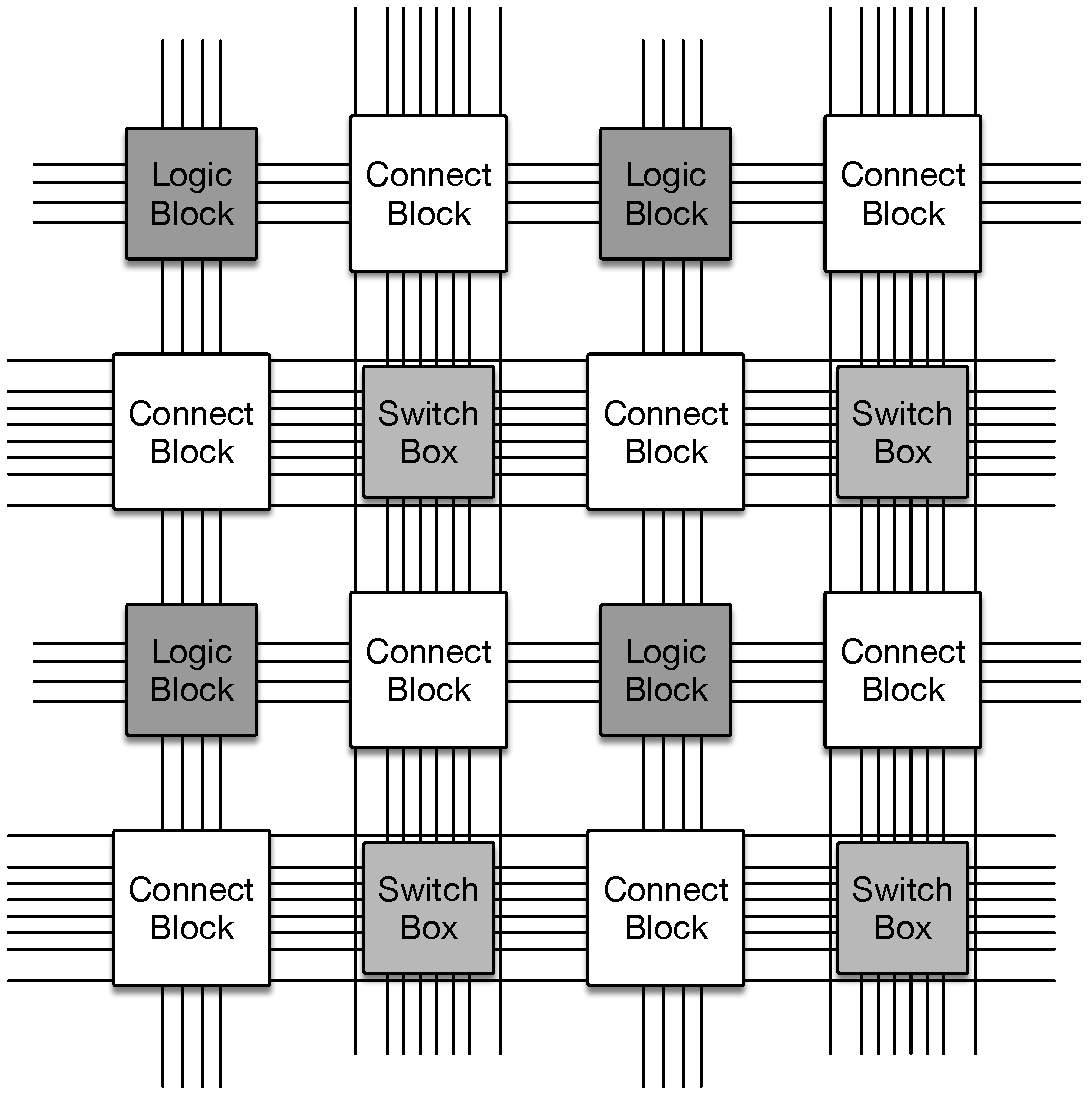
\includegraphics[width=0.6\textwidth]{Figures/island_style}%
    \caption{General island-style FPGA layout. Source:~\cite{ComptonH2002Reconfigurablecomputingsurvey}.}
    \label{fig:island-style_fpga}
\end{figure}

For our explanations, we consider the virtual FPGA structure on two different levels:
\begin{enumerate}
    \item The global structure and layout with all the interconnect between the CLBs.
    \item The local structure and layout within each CLB.
\end{enumerate}

\subsubsection{Global Structure}
The outer, global structure of the generated virtual FPGAs consists of an \(X \times Y\) array of CLBs as depicted in Figure~\ref{fig:global_zuma_structure}.
The inputs and outputs of the virtual device are modeled on the edges of the grid, resulting in \({2 \cdot (X + Y)}\) IO pads.
For ZUMA, each of these IO pads comprises two general purpose IOs, i.e., IOs which can be configured to be either a global input or a global output, such that the virtual device has \({\#GIOs = 4 \cdot (X + Y)}\).
Thus, the overlay can divide the \(\#GIOs\) general purpose IOs between the global inputs and outputs as required by the current circuit.

\begin{figure}[htp]
    \centering
    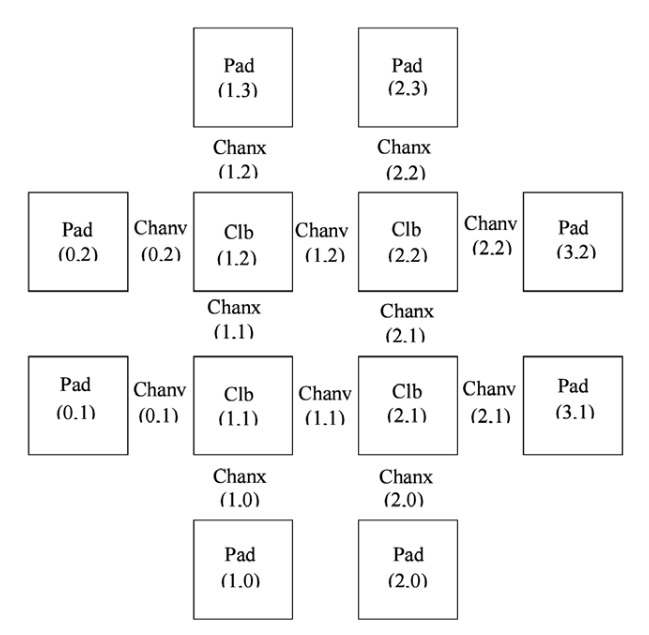
\includegraphics[width=0.6\textwidth]{Figures/structure.pdf}
    \caption{Global structure of a \(2 \times 2\) virtual FPGA. Source: VPR manual.}
    \label{fig:global_zuma_structure}
\end{figure}

\newpage
The routing resources are organized as routing channels in \emph{x} or \emph{y} direction (\emph{Chanx} and \emph{Chany}), and they form a unidirectional interconnect network between the CLBs and the outer IOs.
Each channel consists of a number of individual tracks that can carry one logical signal each.
The channels and tracks are visualized in Figure~\ref{fig:channels}.

\begin{figure}[htpb]
    \centering
    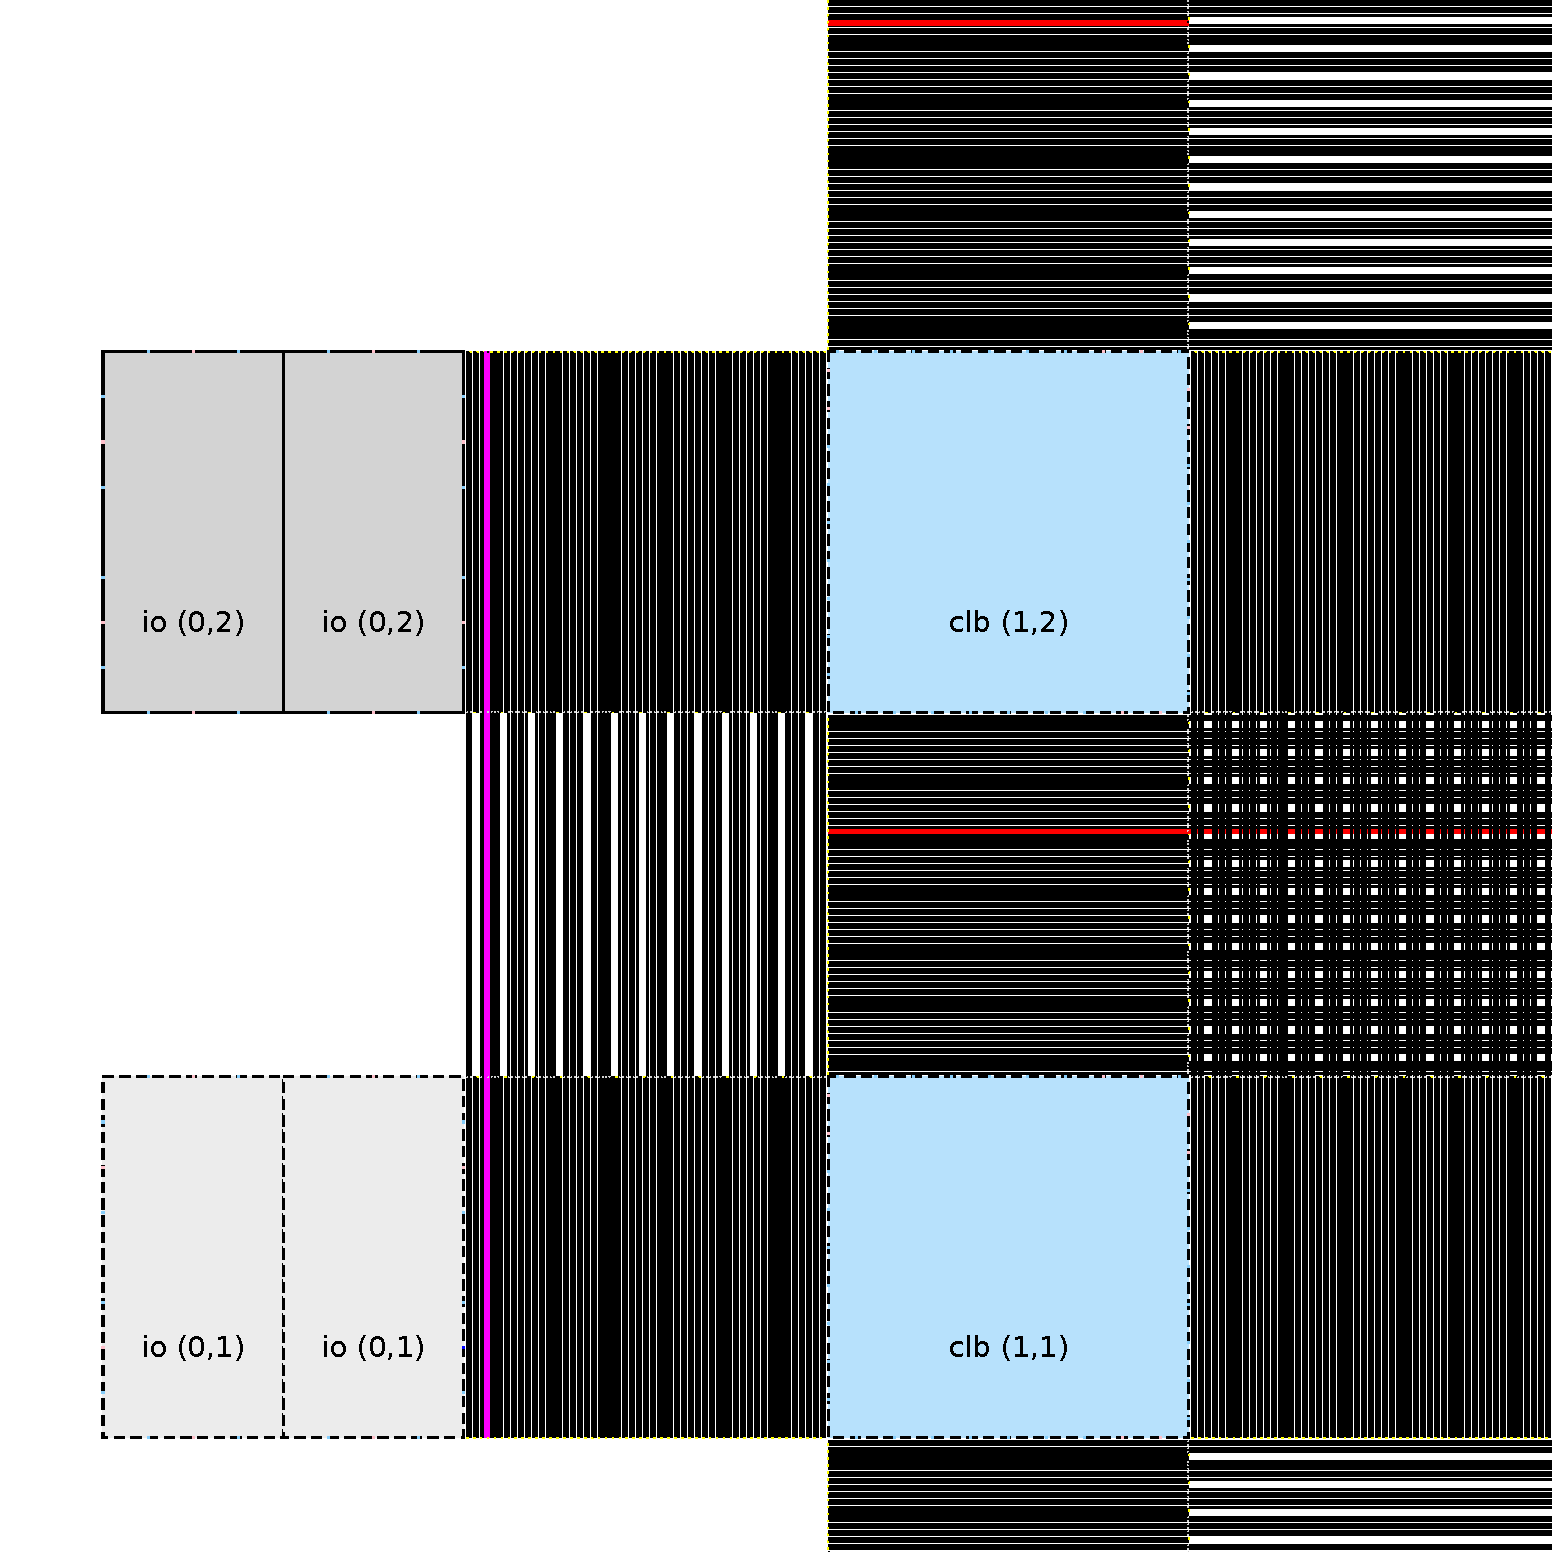
\includegraphics[width=0.6\textwidth]{Figures/channels.pdf}
    \caption{Tracks of different lengths and directions in channels: The purple track connects resources vertically and has a length of 2, while red ones are horizontal and the upper one has a length of 1. Source: VPR.}
    \label{fig:channels}
\end{figure}

\FloatBarrier

The channels are connected to each other via switchboxes,
which are shown in Figure~\ref{fig:switchboxes}.
Within these areas, a selection of tracks from each channel can be connected to a selection of other tracks of different channels.
Since allowing the complete connection of any track to any other track would be too area consuming, ZUMA overlays, like many other FPGA devices, employ a crossbar pattern known as Wilton routing~\cite{wilton1997ArchitecturesandAlgorithms} here.

\begin{figure}[htp]
    \centering
    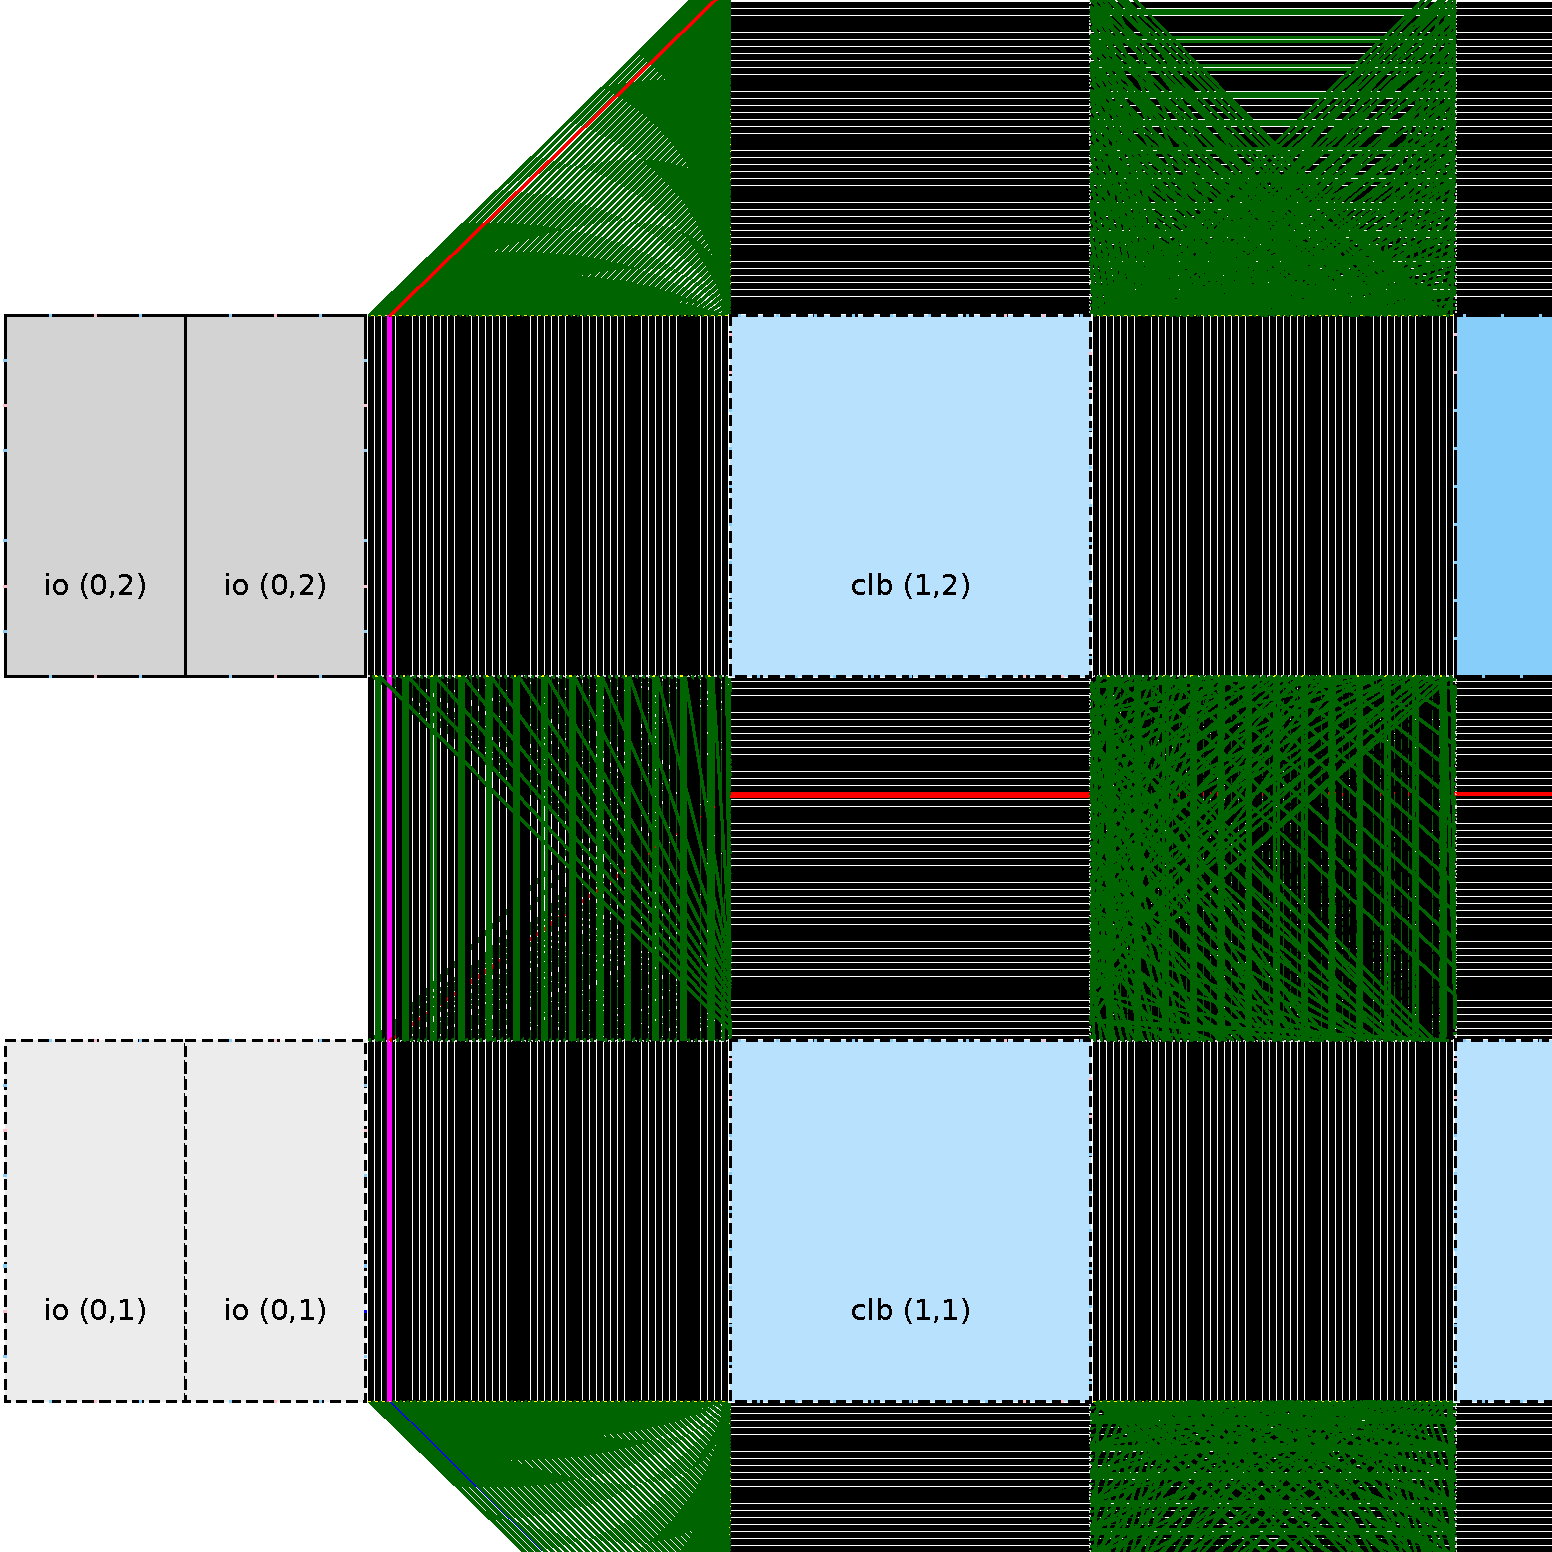
\includegraphics[width=0.6\textwidth]{Figures/switchbox.pdf}
    \caption{Tracks of channels are connected by the switchboxes (green). Source: VPR.}
    \label{fig:switchboxes}
\end{figure}

Each CLB connects to some of the tracks of the surrounding channels of the global routing resources -- these connection locations are typically called connect blocks (cp.~Figure~\ref{fig:island-style_fpga}).
Each CLB element thus has its own connect block to connect itself to the global routing resources, and a switchbox to actually realize the global routing.
Therefore the global outer structure of a ZUMA virtual FPGA consists of the global routing network (channels, connect blocks, and switchboxes), CLBs (or clusters), and IO pads.

\FloatBarrier
\subsubsection{Local Structure}
Each CLB, or cluster, consists of an input interconnect block (IIB) for its intra-cluster input routing and \(N\) basic logic elements (BLE).
These BLEs in turn comprise one lookup table (LUT) with input width K, and one flip flop (FF) that is bypassable using a configurable MUX, see image \ref{fig:cluster}.

\begin{figure}[htbp]
    \centering
    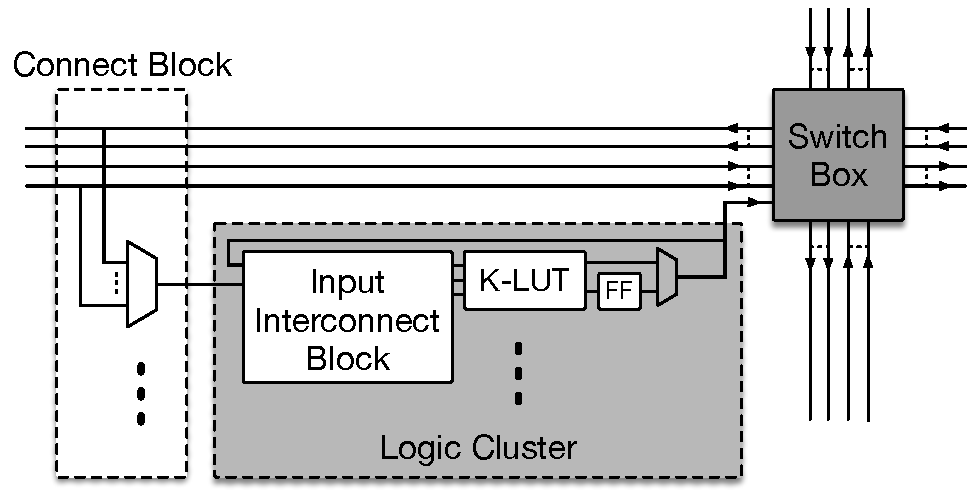
\includegraphics[width=0.7\textwidth]{Figures/ZUMA_CLB}
    \caption{The structure of a ZUMA CLB, or cluster.}
    \label{fig:cluster}
\end{figure}

The \(N\)\,bit output of the whole cluster is the combined output of the \(N\) individual BLEs.
The IIB is fed with the \(I\) inputs from the connect block, i.e., the connected input tracks from the global routing resources, and also with the \(N\) feedback outputs from the BLE elements.
Each of these \({(I+N)}\) inputs must be routed to (almost) every pin of all \(N\) LUTs.
Therefore the \({N \cdot K}\) outputs of the IIB are connected to the different input pins of the BLE elements.

\newpage
Currently the IIB is implemented using connected MUXes, and there are two different implementations available to choose from, each with a different MUX density:
\begin{enumerate}
    \item The first IIB is a straightforward fully-connected crossbar between the \({(I+N)}\) inputs and the \({N \cdot K}\) outputs, which requires a considerable amount of MUXes to realize, but cannot suffer from congestion and is thus guaranteed to find a local routing for any configuration.
    \item The second one is based on Clos networks~\cite{Clos1953Studynonblocking} and uses fewer MUXes,
    but the local routing algorithm does not always find a valid interconnect routing, due to randomness in the current routing approach.
\end{enumerate}

\subsubsection{Structure Configuration Parameters}
The structure-related ZUMA configuration parameters are thus as follows:\\[1.5mm]
\renewcommand{\arraystretch}{1.2}%
\begin{tabularx}{\textwidth}{lX}
    \hline
    \multicolumn{2}{l}{\emph{Global structure}} \\
    \hline
    \configvalue{X}             & Grid size in \emph{x} dimension \\
    \configvalue{Y}             & Grid size in \emph{y} dimension \\
    \configvalue{L}             & Length of the routing channels \\
    \configvalue{W}             & Number of tracks per routing channel \\
    \hline
    \multicolumn{2}{l}{\emph{Local structure}} \\
    \hline
    \configvalue{I}             & External cluster inputs (from connect block to IIB) \\
    \configvalue{N}             & LUTs per cluster \\
    \configvalue{K}             & LUT input width \\
    \configvalue{UseClos}       & Whether the IIB should be Clos network-based (otherwise it is a fully connected crossbar) \\
    \cline{1-1}
    \multicolumn{2}{l}{\emph{Connect block}} \\
    \cline{1-1}
    \configvalue{fc_in}        & From how many tracks of the connect block each of the \(I\) cluster inputs can be driven \\
    \configvalue{fc_in_type}  & Whether \configvalue{fc_in} is an absolute number or relative value \\
    \configvalue{fc_out}       & How many tracks of the connect block each of the \(N\) cluster outputs can drive\\
    \configvalue{fc_out_type} & Whether \configvalue{fc_out} is an absolute number or relative value \\
    \hline \\
\end{tabularx}

\subsubsection{Data Structures}
\label{ssub:basic_model_structure_data_structures}
The whole virtual FPGA structure is saved in different data structures, whose scope and purpose we will briefly discuss here.

Within the VTR flow, the overall layout and the local structure are stored in an XML architecture description file, e.g., \inlinepath{ARCH.xml}.
The expanded global structure of the FPGA is stored in the routing resource graph (RRG), which is also an XML file in VTR8, e.g., \inlinepath{rr_graph.xml}.

Within ZUMA, the whole structure is built into one complete graph, let us call it overlay description graph (ODG) here for easier reference. This ODG includes all virtual resources and structures, i.e., IO pads, routing MUXes, eLUTs, and FFs. To be able to use Xilinx' LUTRAM macros of a specific input width \(l\) (or the Altera alternative) to implement the overlay later, the ODG has to be made \(l\)-feasible, i.e., each node must have a fan-in of at most \(l\) and a fan-out of exactly \(1\). This process is one of the internal processes within the overlay generation, and the resulting \(l\)-feasible ODG is used for most processing steps within the flow. Within the rest of this document, we will call the former graph the ODG, and the latter one the technology-mapped ODG.




\subsection{ZUMA Tool Flow Details}
\label{sub:zuma_flow_details}
To fully understand all generated files, we have to take a closer look into the inner workings of the ZUMA overlay generation, which we will do in this section.
These are thus the flow details that happen automatically when running \command{compile.sh}.

\subsubsection{Basic Flow}
\label{ssub:ZUMA_flow_details_basic}
The detailed steps to generate an overlay using the flow depicted in Figure~\ref{fig:zumaflow} are as follows for the basic version without timing analysis or optimization (user interaction is only required for top-level items):
\begin{enumerate}
    \item Set all values in \inlinepath{zuma_config.py} to fit your needs.
    \item Run the ZUMA flow (\inlinepath{compile.sh} with your virtual circuit).
    \begin{enumerate}
        \item \inlinepath{generate_buildfiles.py}
        \begin{itemize}
            \item Generates the VPR architecture files and build scripts from templates, i.e., currently \inlinepath{ARCH_vpr8.xml}, \inlinepath{abccommands.vpr8}, \inlinepath{vpr8.sh}, and \inlinepath{vpr8_timing.sh} in the \inlinepath{build} directory, or their VPR 7 alternatives.
            \item Applies the parameters from \inlinepath{zuma_config.py} to all generated files.
        \end{itemize}
        \item \command{VTR}
        \begin{itemize}
            \item Synthesizes the virtual circuit into a technology-mapped BLIF file.
            \item Generates all local and global routing resources in VPR.
            \item Saves the global ones as routing resource graph (RRG).
            \item Saves the result of its packing, placement and routing steps as a netlist, placement and routing file.
        \end{itemize}
        \item \inlinepath{zuma_build.py}
        \begin{itemize}
            \item Parses the global routing resources from the RRG.
            \item Builds up an internal overlay description graph (ODG, cp.~Section~\ref{ssub:basic_model_structure_data_structures}) representing all global and local resources from the parsed global information and statically for the local ones.
            \item Builds the technology-mapped ODG from the ODG by expanding nodes which use too many inputs to fit into the targeted LUTRAM macros.
            \item Writes out the Verilog description for the complete overlay by going through all nodes and edges of the technology-mapped ODG and generating a correspondingly connected LUTRAM instantiation in Verilog.
            \item Parses the information from the BLIF, netlist, placement, and routing files and correlates it with the technology-mapped ODG, i.e., which LUT node implements which functionality, which signal name is used where, how do the routing nodes need to be configured to pass along the signals the correct way, etc.
            \item Builds the ZUMA bitstream for the virtual circuit by going through all nodes of the technology-mapped ODG and saving their configuration as the corresponding LUTRAM configuration.
        \end{itemize}
        \item Verifies whether the generated circuit is functionally equivalent to the original specification.
    \end{enumerate}
    \item Include the generated overlay in an FPGA design (cf.~Section~\ref{sec:include_ZUMA_in_project}).
    \item Run the device vendor's EDA tools.
    \item Configure the ZUMA overlay with the bitstream.
\end{enumerate}




\subsubsection{Timing-augmented Flow}
\label{ssub:ZUMA_flow_details_timingdriven}
\emph{Note}: This section is currently only applicable to Xilinx devices.

\noindent The detailed steps to generate an overlay using the flow depicted in Figure~\ref{fig:zumaflow} are as follows for the version with all bells and whistles, which allows for static timing analysis of the virtual circuit mapped to the physical device, as well as timing-driven virtual placement and routing.
For the steps that are already part of the details presented in Section~\ref{ssub:ZUMA_flow_details_basic}, we only give reduced details here, to focus on the differences (user interaction is again only required for top-level items, except for the SDF extraction):
\begin{enumerate}
    \item \label{enum:first_td_pnr_new_overlay_subflow} Set all values in \inlinepath{zuma_config.py} to fit your needs.
    \item Set \configvalue{vprAnnotation} = False and \configvalue{sdf} = False in \inlinepath{zuma_config.py}.
    \item Run the ZUMA flow (\inlinepath{compile.sh} with dummy\,/\,any virtual circuit).
    \begin{enumerate}
        \item \inlinepath{generate_buildfiles.py}
        \item \command{VTR} (with timing analysis off)
        \item \inlinepath{zuma_build.py}
        \begin{itemize}
            \item Writes out the Verilog description for the complete overlay.
        \end{itemize}
    \end{enumerate}
    \item Include the generated overlay in an FPGA design (cf.~Section~\ref{sec:include_ZUMA_in_project}).
    \item Run the device vendor's EDA tools.
    \item \label{enum:last_td_pnr_new_overlay_subflow} Extract and copy the standard delay format (SDF) file(s) describing the timing properties of the overlay.
    \begin{itemize}
        \item For Vivado, generate the SDF file that contains the routing delay information by opening your top-level design and issuing the following command in the tcl console:
\begin{verbatim}
>write_sdf Top_complete.sdf
\end{verbatim}
              Copy the generated file \inlinepath{Top_complete.sdf} to your \inlinepath{example/} directory.
              Edit the parameter \configvalue{sdfFileName} to this name in \inlinepath{zuma_config.py} (The parameter \configvalue{sdfFlipflopFileName} is not used in the vivado flow).
        \item For ISE, also assuming that your top-level design has the name \emph{Top}, generate the first SDF file that contains the the routing delay information by issuing:
\begin{verbatim}
>netgen -s 1  -pcf Top.pcf -sdf_anno true -sdf_path "netgen/par" \
-ne -insert_glbl true -insert_pp_buffers false -w \
-dir netgen/par -ofmt verilog -sim Top.ncd Top_no_buffer.v
\end{verbatim}
        And then generate the second SDF file that holds the flip flop delays (port delay + Tshcko) like this:
\begin{verbatim}
>netgen -s 1  -pcf Top.pcf -sdf_anno true -sdf_path "netgen/par" \
-ne -insert_glbl true -insert_pp_buffers true -w \
-dir netgen/par -ofmt verilog -sim Top.ncd Top_with_buffer.v
\end{verbatim}
        Copy the generated file(s) \inlinepath{Top_with_buffer.sdf} and \inlinepath{Top_no_buffer.sdf}, if applicable, to your \inlinepath{example/} directory.
        Edit the parameters \configvalue{sdfFileName}, and \configvalue{sdfFlipflopFileName} to these names in \inlinepath{zuma_config.py}.
    \end{itemize}
    \item \label{enum:first_td_pnr_new_circuit_subflow} Set \configvalue{vprAnnotation} = True and \configvalue{sdf} = True in \inlinepath{zuma_config.py}.
    \item Run the ZUMA flow for a second time (\inlinepath{compile.sh} with your actual virtual circuit) -- or multiple times thereafter for new virtual circuits.
          This will invoke two different subflows which will be explained in the following.
    \item Subflow 1:
    \begin{enumerate}
        \item \inlinepath{generate_buildfiles.py}
        \begin{itemize}
        	\item Generates \inlinepath{ARCH_vpr8.xml}, \inlinepath{abccommands.vpr8}, \inlinepath{vpr8.sh}, and \inlinepath{vpr8_timing.sh} in the \inlinepath{build} directory.
        	\item Within \inlinepath{ARCH_vpr8.xml}, every CLB and BLE are their own individual instance with zeroed timing.
        \end{itemize}
        \item \command{VTR} (with timing analysis off)
        \item \inlinepath{zuma_build.py}
        \begin{enumerate}
            \item \inlinepath{ReadSDF.py}
            \begin{itemize}
                \item Parses the SDF file, identifies mappings of SDF cells and technology-mapped ODG (cp.~Section~\ref{ssub:basic_model_structure_data_structures}) nodes and augments the ODG with the timing information for routing MUXes and LUTs (\command{addLutCellDelayToMappedNode}), as well as FFs (\command{addFlipflopCellDelayToMappedNode}).
                \item Parses iopath and read port delays, as well as setup and hold times.
                \item Parses only worst-case times, as VPR can only handle one delay entry per entity, and the worst case is then usually the most interesting one.
            \end{itemize}
            \item \inlinepath{TimingAnalysisSDF.py} \command{performTimingAnalysis()} calculates the critical path from the delay-augmented technology-mapped ODG.
            \item \inlinepath{NodeGraphTiming.py}
            \begin{itemize}
                \item Computes the delay information of the ODG nodes from the imported information in the technology-mapped ODG nodes, i.e., congregates the delay of expanded nodes into a delay for their supernode.
                \item This step is necessary, as only the nodes of the original ODG correspond to the entities known to VPR.
            \end{itemize}
            \item \inlinepath{TimingAnnotation.py} \command{annotateClusterTiming()}
            \begin{itemize}
                \item Computes delays of all paths within the clusters which connect entities to each other that are known to VPR.
            \end{itemize}
            \item \inlinepath{TimingAnnotation.py} \command{annotateBack()} writes all computed delays from the augmented (original) ODG into the files \inlinepath{ARCH_vpr8_timing.xml} and \inlinepath{rr_graph_timing.xml}.
        \end{enumerate}
    \end{enumerate}
    \item Subflow 2:
    \begin{enumerate}
        \item \inlinepath{generate_buildfiles.py}
        \item \command{VTR}
        \begin{itemize}
             \item Now using \inlinepath{vpr8_timing.sh} and thus with timing analysis on.
             \item Uses the delay-augmented \inlinepath{ARCH_vpr8_timing.xml} and \inlinepath{rr_graph_timing.xml}.
             \item Can thus perform (meaningful) timing-driven placement and routing.
         \end{itemize}
        \item \inlinepath{zuma_build.py}
        \begin{enumerate}
            \item Now uses \inlinepath{rr_graph_timing.xml} and RRG.
            \item \inlinepath{ReadSDF.py}
            \item \inlinepath{TimingAnalysisSDF.py} \command{performTimingAnalysis()} can now do a proper timing analysis for the current virtual circuit, giving a delay estimate with a corresponding maximum frequency \(f_{max}\).
            \item Builds the ZUMA bitstream for the virtual circuit.
        \end{enumerate}
    \end{enumerate}
    \item Set the clock for the virtual device to a frequency \(\leq f_{max}\).
    \item \label{enum:last_td_pnr_new_circuit_subflow} Configure the ZUMA overlay with the bitstream.
\end{enumerate}

After performing these steps, you can run the ZUMA \inlinepath{compile.sh} script with any virtual circuit to get its critical path. The path and resulting frequency \(f_{max}\) will be printed on the command line.
To create a new timing-augmented overlay, repeat steps \ref{enum:first_td_pnr_new_overlay_subflow} through \ref{enum:last_td_pnr_new_overlay_subflow}, to just map a new virtual circuit to an existing overlay, repeat steps \ref{enum:first_td_pnr_new_circuit_subflow} through \ref{enum:last_td_pnr_new_circuit_subflow}.

\subsection{Generated Data Structures and Files}
\label{sub:data_structures_and_files_visualization}
In this section we will now give an overview of the intermediate and final generated files and data structures.

For thorough descriptions of the architecture\footnote{Architecture: \url{https://docs.verilogtorouting.org/en/latest/arch/}} and routing resource graph\footnote{RRG: \VTRdocRRG} files, see the documentation of the VTR flow.

\subsubsection{Overlay Description Graph}
The first own data structure of the ZUMA flow is the ODG, the internal representation of all resources of the virtual FPGA.
It is generated in two steps:
\begin{enumerate}
    \item The global, outer structure of the virtual FPGA is generated from the RRG, consisting of the global routing network (channels and switchboxes) and clusters, but not the inner structure within such a cluster.
    \item The inner structure of the different clusters (BLE elements and interconnect routing) is created from scratch analogously to the architecture file.
\end{enumerate}

%\subsubsubsection{build outer structure}
For the first step, Figure~\ref{fig:outer_structure_small} shows an example of such an outer structure.
\begin{figure}[htbp]
    \centering
    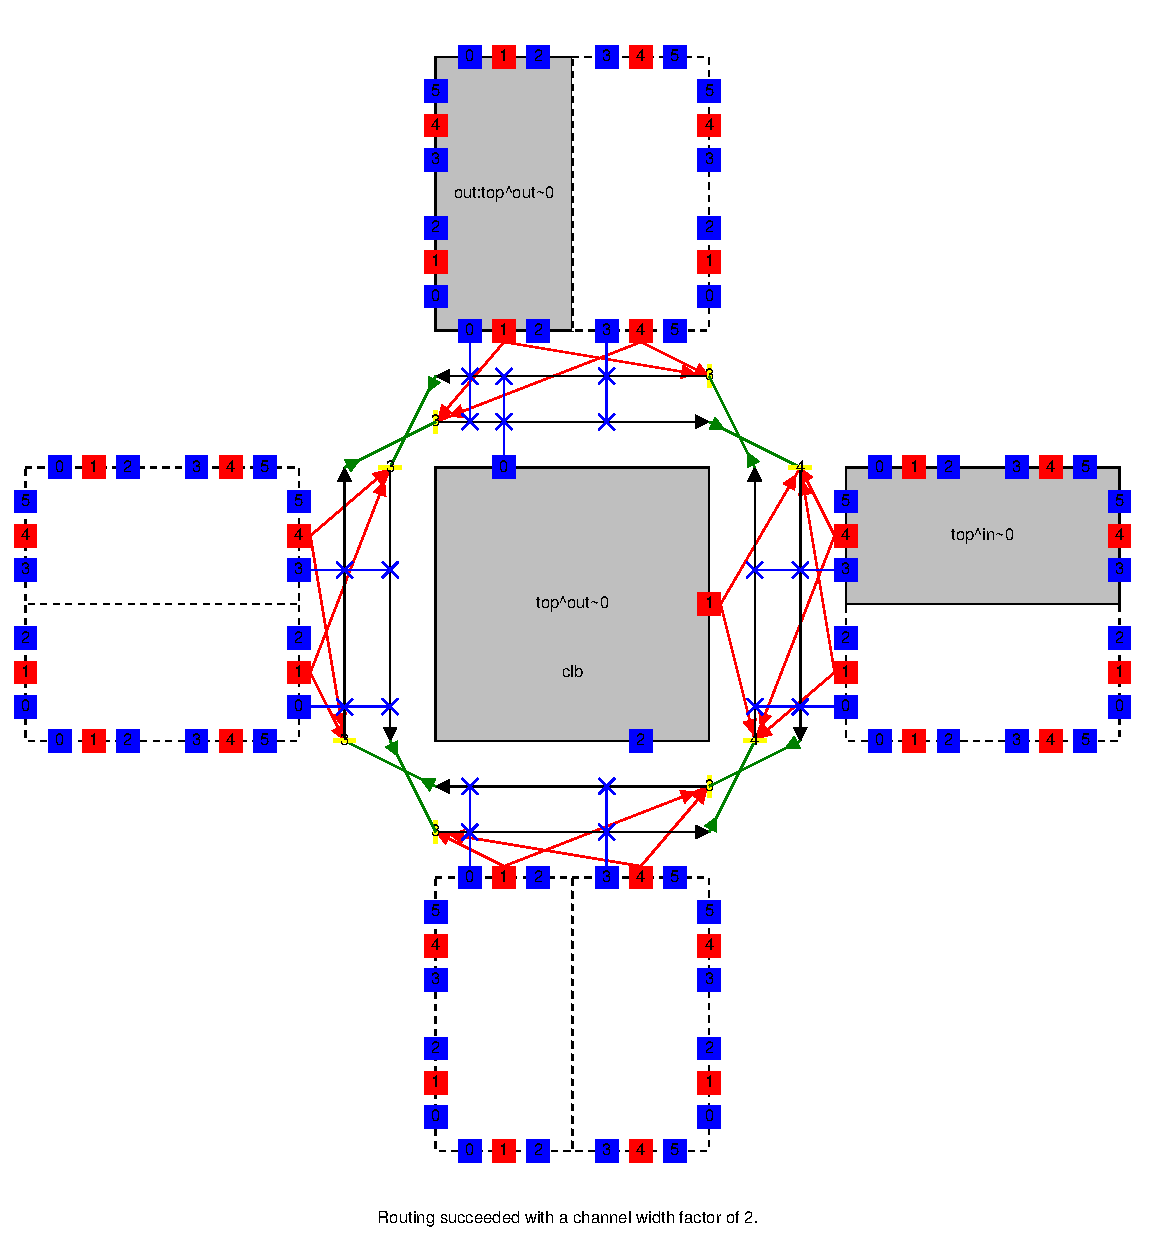
\includegraphics[width=.7\textwidth]{Figures/unconfigured.pdf}
    \caption{A small outer structure: We have 8 channels of length one (black arrows), 8 output pins (OPIN, red numbered blocks) on the IO pad which route the input of an fpga. We have 8 input pins(IPIN, blue numbered blocks) on the IO pads, which route to the output of the fpga. We have one used cluster input (IPIN, blue) and one output pin (OPIN,red). Also we have switchbox connections (green arrows).}
    \label{fig:outer_structure_small}
\end{figure}
To get such a structure the script parses the RRG file generated by VPR, which contains the outer structure visualized in Figure~\ref{fig:outer_structure_small} as a graph.
We load this RRG in the function \command{load_graph(filename)} in the file \inlinepath{InitFpga.py}.
%\subsubsubsection{build inner structure}
Because we can only obtain the outer, global structure from it, we have to add the nodes for the inner, local structure ourselves. In our example this only affects the cluster location 1\_1.
Figure~\ref{fig:cluster_loaded} shows the original cluster, while the updated cluster is shown in Figure~\ref{fig:cluster_added_nodes}.
\begin{figure}[htbp]
    \centering
    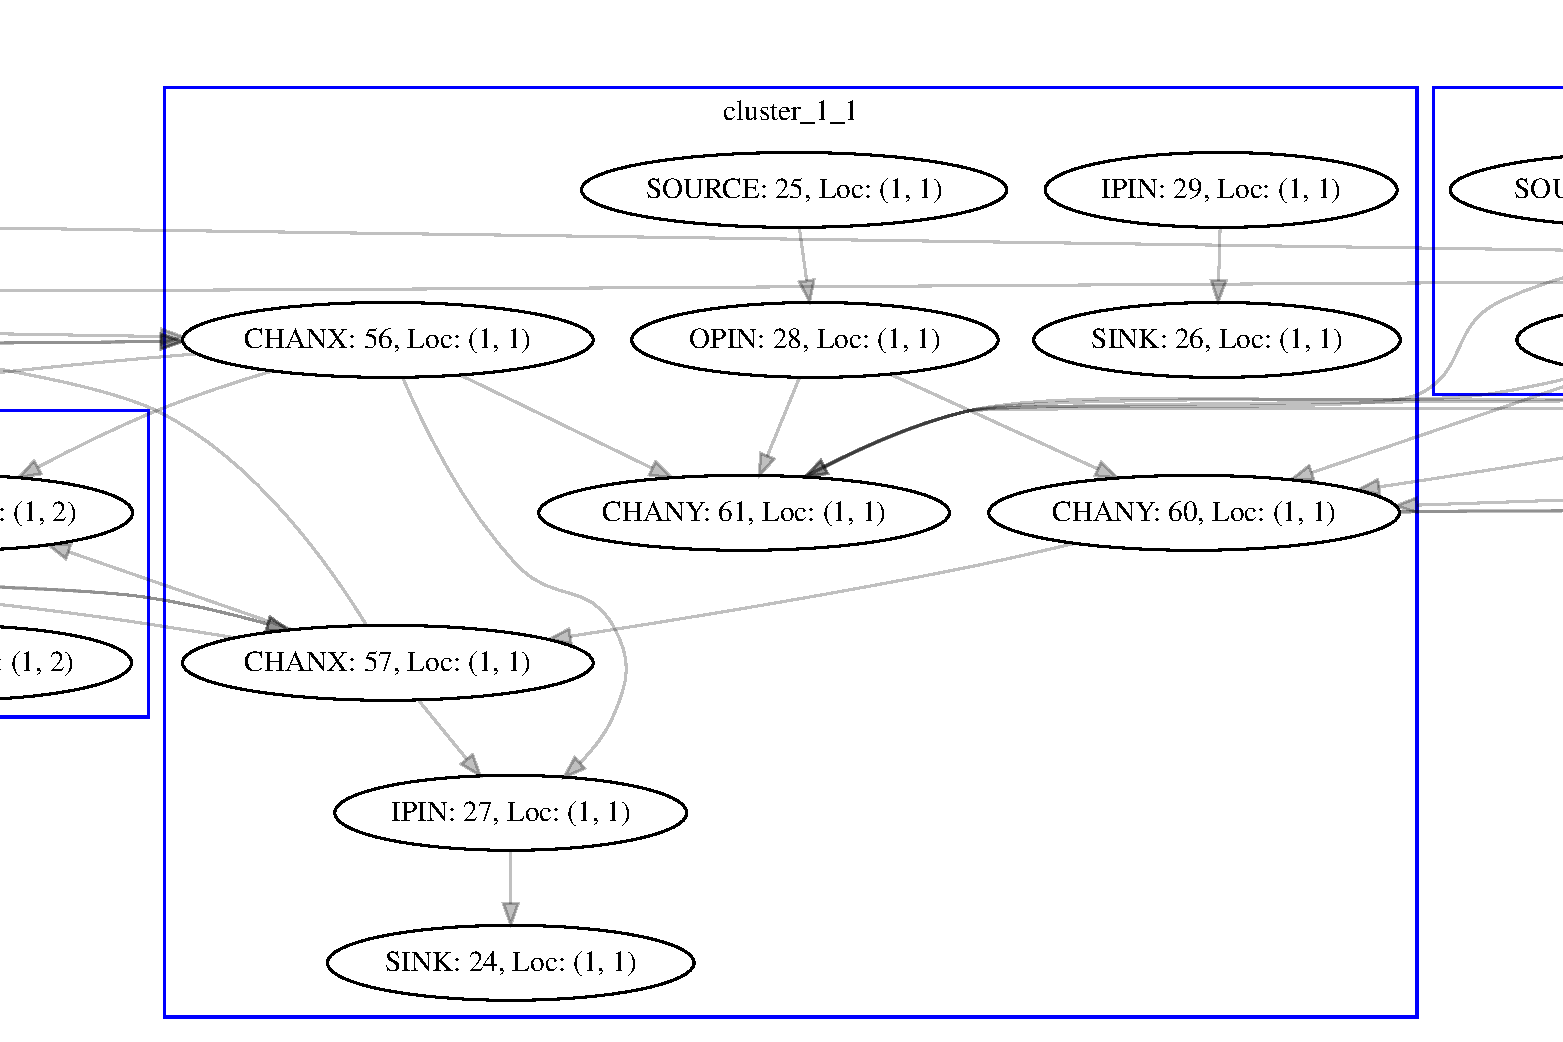
\includegraphics[width=\textwidth]{Figures/loadedGraphcutted.pdf}
    \caption{An overlay description graph, after the RRG parsing.}
    \label{fig:cluster_loaded}
\end{figure}
\begin{figure}[htbp]
    \centering
    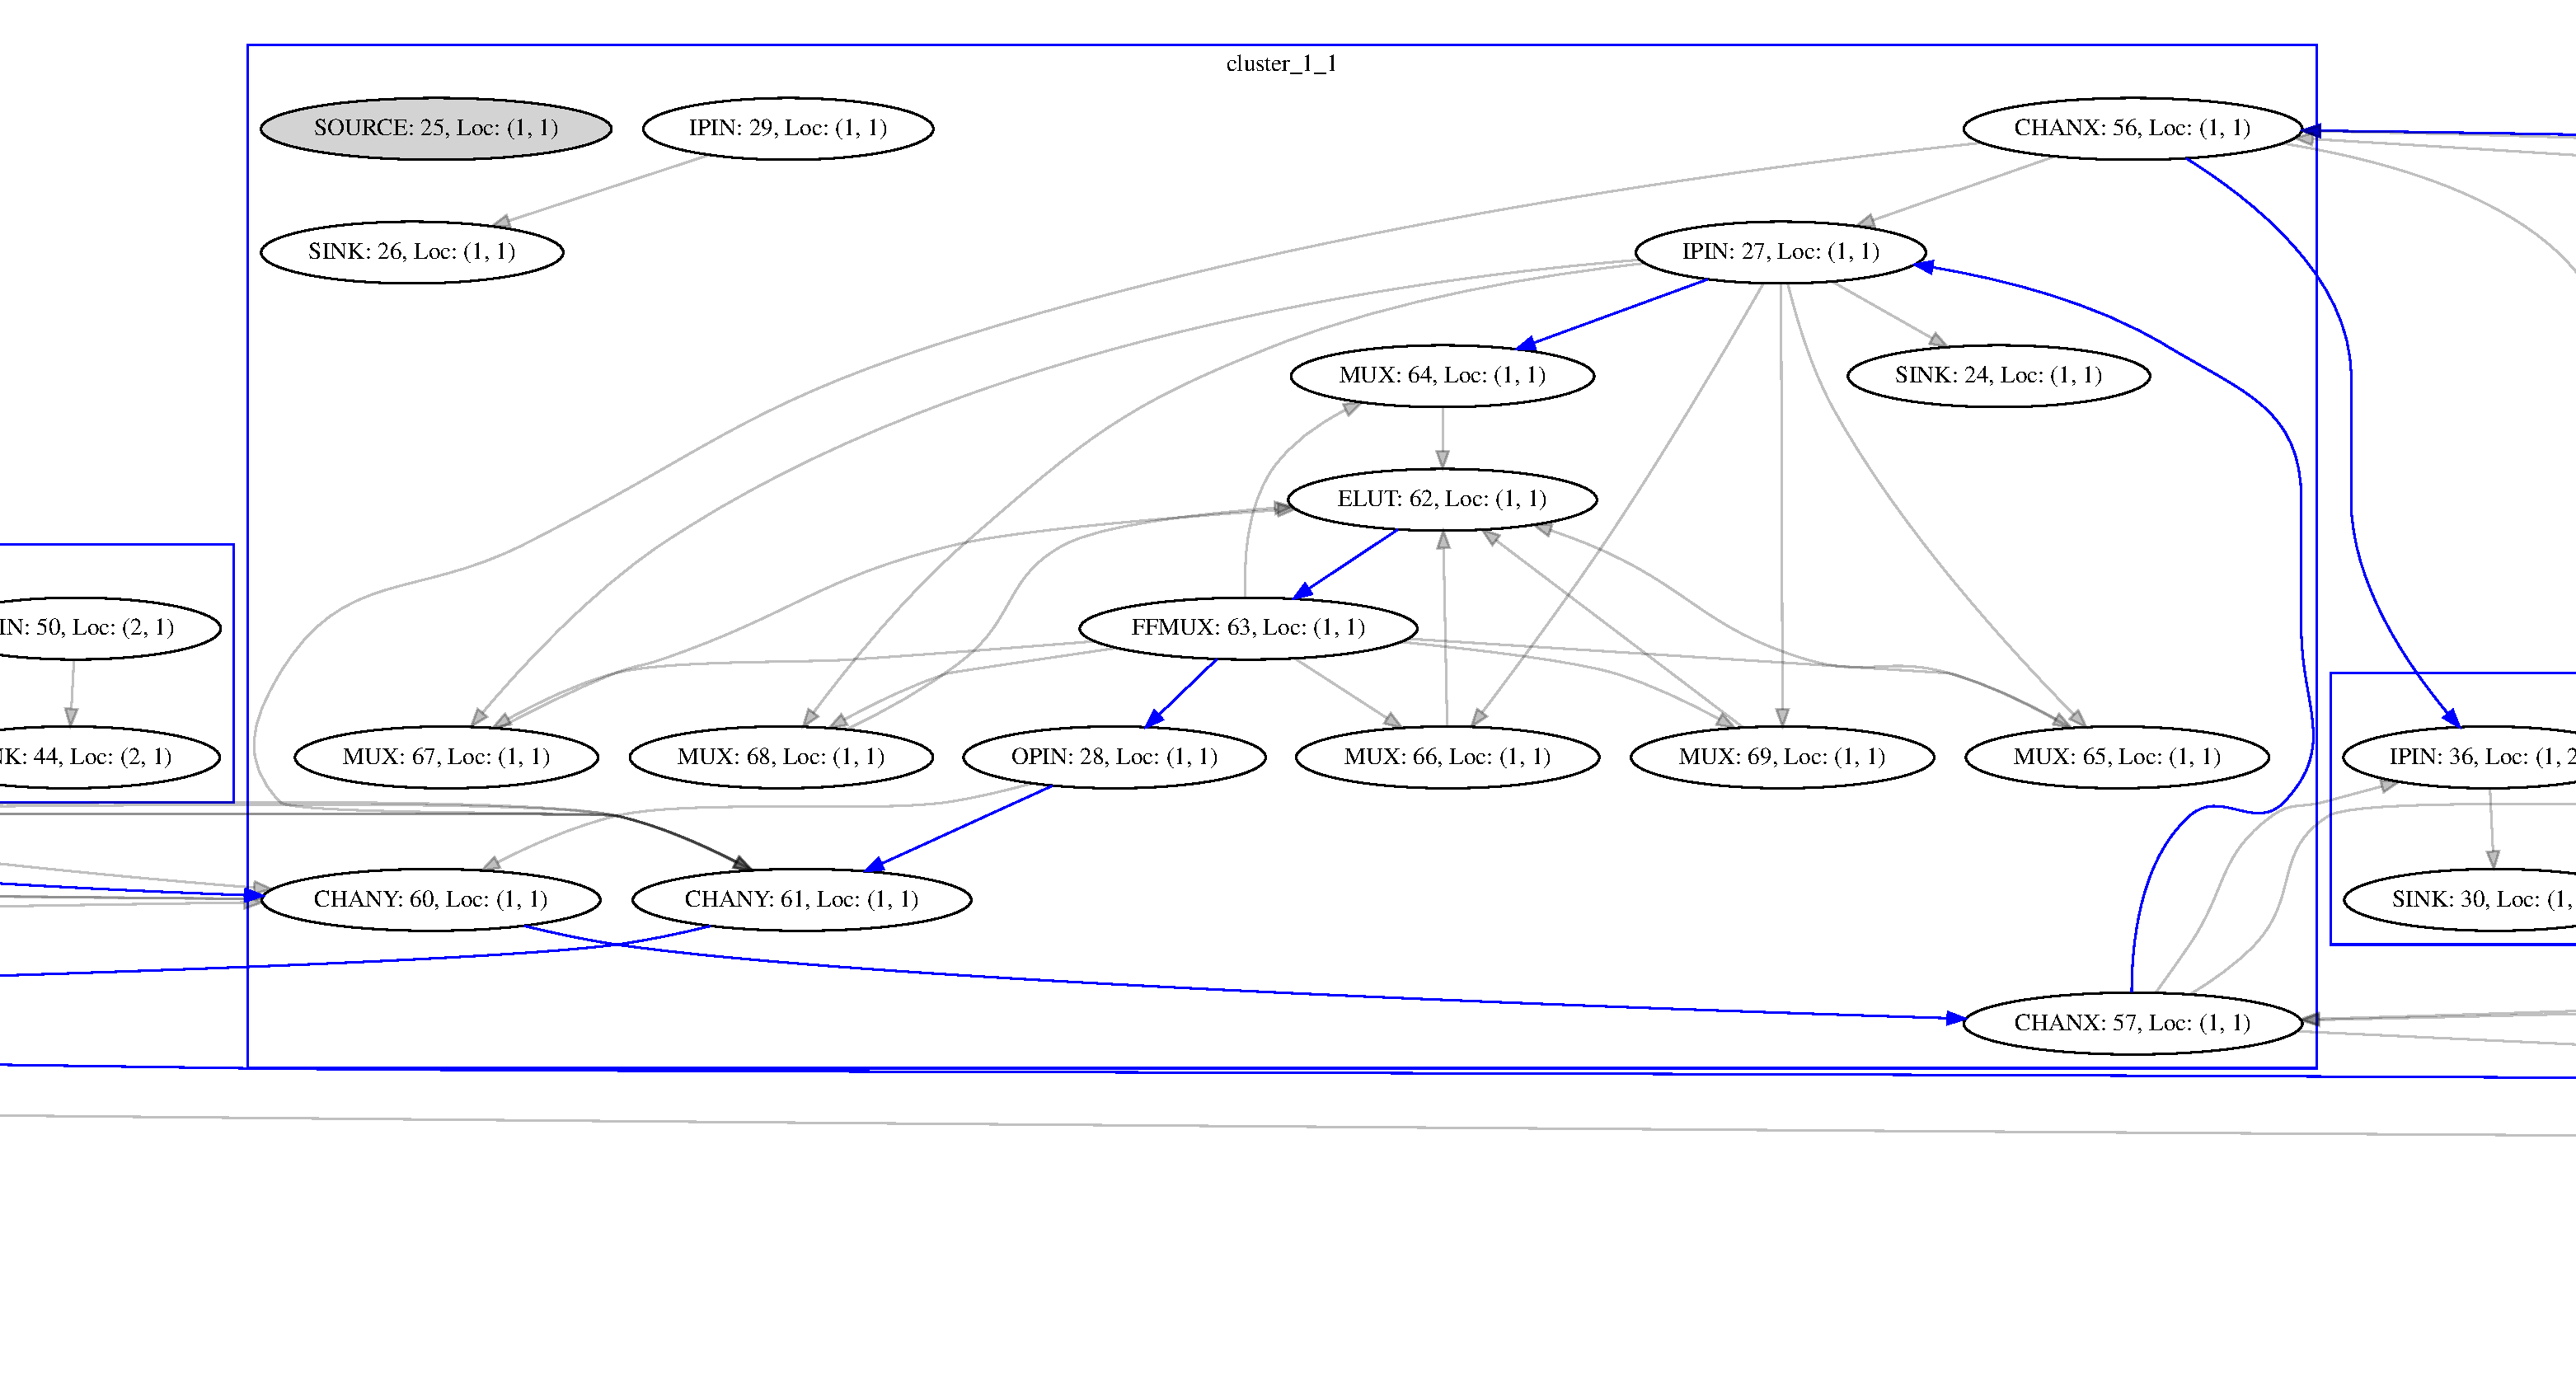
\includegraphics[width=\textwidth]{Figures/originGraphcutted.pdf}
    \caption{An ODG with added nodes for the local structure.}
    \label{fig:cluster_added_nodes}
\end{figure}
The graph was altered by the following steps of the function \command{build_inner_structure()} in the file \inlinepath{InitFpga.py}:
\begin{enumerate}
    \item For each BLE add an eLUT (node 62) and a MUX (63), which decides whether the flip flop of that BLE is bypassed or not. The FF does not have to be added as a separate node as the eLUT and FF are grouped together into one entity for the generated Verilog file. Connect the new nodes appropriately.
    \item Connect the MUX output with the cluster output pin (28) for routing the signal out of the cluster. To this end, we dismount the OPIN from the source node (25) because this node is not useful anymore and will be removed in the build of the Verilog file.
    \item Add the nodes for the IIB in the function \command{buildSimpleNetwork()}: Add enough MUXes to route the cluster inputs and the BLE outputs to every pin of every LUT. Therefore each pin gets its own MUX (64 - 69) and the inputs of these MUXes are the cluster input node (27) and the output of the one LUT MUX (63).
\end{enumerate}

Furthermore we have to generate a \(k_{host}\)-feasible version of the ODG, i.e., we have to replace each node with more than \(k_{host}\) input edges (more than \(k_{host}\) pins) with several nodes, because the real FPGA hardware we want to synthesize our virtual FPGA on, has only \(k_{host}\) pins per LUT.
\(k_{host}\) is implemented as global constant \parameter{globs.host_size}~=~6.

The generation of the possible LUT types is realized in:
\begin{itemize}
    \item writeSimpleLut()
    \item writeTightlyLut()
    \item writeComplexLut()
\end{itemize}

In this document, we call this new, expanded overlay description graph the technology-mapped ODG.

\FloatBarrier

\subsubsection{Verilog file}
The central Verilog file \inlinepath{ZUMA_custom_generated.v}, which describes the complete configurable overlay, is generated in the function \command{build_global_routing_Verilog} in the file \inlinepath{BuildVerilog.py}.
As explained before, the basic approach is to traverse the ODG and write its structure into a file, translated to Verilog primitives and Xilinx macros.
We also perform several optimizations to omit the generation of useless nodes, which:
\begin{itemize}
    \item Are sources/sink nodes,
    \item have no input, or
    \item have only one input, i.e., passthrough nodes. For these, we use Verilog assigns instead of generating routing MUXes. An exception are FF MUXes, because they will have two inputs on the real FPGA hardware, but not in our graph.
\end{itemize}

Listing~\ref{lst:verilog_ZUMA_custom_generated.v} shows an example excerpt of a generated Verilog file, with some of the interesting elements:
\begin{itemize}
    \item The outward Verilog module interface (which we will discuss in a later section).
    \item ODG nodes that are translated to wires.
    \item Passthrough nodes from the ODG that are realized using Verilog assigns.
    \item A LUTRAM macro instantiation for a routing MUX (\hwport{mux_337}).
    \item A LUTRAM macro instantiation for an eLUT (\hwport{c_mux_1316}) and its FF MUX (\hwport{c_mux_1317}).
    \item The IO pad endpoints \hwport{fpga_outputs[i]} and \hwport{fpga_inputs[i]}.
    \item The instantiation of the simple configuration controller.
\end{itemize}

\begin{lstlisting}[style=Verilog,caption={{Example Verilog excerpt from ZUMA\_custom\_generated.v.}}, label={lst:verilog_ZUMA_custom_generated.v}]
    `include "define.v"
    //ZUMA global routing Entity
    //automatically generated by script
    module ZUMA_custom_generated
    #(
        parameter N_NUMLUTS = 8,
        parameter I_CLINPUTS = 28,
        parameter K_LUTSIZE  = 6,
        parameter CONFIG_WIDTH  = 32
     )
    (
    clk,
    fpga_inputs,
    fpga_outputs,
    config_data,
    config_en,
    progress,
    config_addr,
    clk2,
    ffrst
    );
        // [..]
        wire node_0;
        wire node_1;
        wire node_2;
        wire node_3;
        wire node_4;
        // [..]
        //sbox driver x at  (1, 2, 2, 2)
        assign node_836 = node_986;
        //sbox driver x at  (1, 2, 2, 2)
        assign node_837 = node_1298;
        // [..]


        //cluster input at (2, 1)
        //size: 6
        //inputs: [536, 537, 604, 605, 648, 649]
        lut_custom mux_337 (
            .a(wr_addr), // input [5 : 0] a
            .d(wr_data[5]), // input [0 : 0]
            .dpra({node_536,node_537,node_604,node_605,node_648,node_649}), // input [5 : 0] dpra
            .clk(clk), // input clk
            .we(wren[4]), // input we
            .dpo(node_337));

        // [..]

        //internal cluster node (eLUT) at  (1, 2)
        //size: 6
        //inputs: [1332, 1333, 1334, 1335, 1336, 1337]
        elut_custom c_mux_1316 (
            .a(wr_addr), // input [5 : 0] a
            .d(wr_data[11]), // input [0 : 0]
            .dpra({node_1332,node_1333,node_1334,node_1335,node_1336,node_1337}), // input [5 : 0] dpra
            .clk(clk), // input clk
            .we(wren[27]), // input we
            .dpo(node_1316_unreg), // unregistered output
            .qdpo_clk(clk2), // run clk
            .qdpo_rst(ffrst), // input flip flop reset
            .qdpo(node_1316_reg)); // registered output

        //internal cluster node (ffmux) at  (1, 2)
        //size: 1
        //inputs: [1316]
        lut_custom c_mux_1317 (
            .a(wr_addr), // input [5 : 0] a
            .d(wr_data[12]), // input [0 : 0]
            .dpra({node_1316_reg,node_1316_unreg,1'b0,1'b0,1'b0,1'b0}), // input [5 : 0] dpra
            .clk(clk), // input clk
            .we(wren[27]), // input we
            .dpo(node_1317));

        // [..]

        assign fpga_outputs[0] = node_0;
        assign fpga_outputs[1] = node_3;
        // More of these
        assign node_1 = fpga_inputs[0];
        assign node_4 = fpga_inputs[1];
        // More of these
        parameter NUM_CONFIG_STAGES = 78;
        config_controller_simple
        #(
            .WIDTH(CONFIG_WIDTH),
            .STAGES(NUM_CONFIG_STAGES),
            .LUTSIZE(K_LUTSIZE)
        )
        configuration_ctrl
        (
            .clk(clk),
            .reset(1'b0),
            .wren_out(wren),
            .progress(progress),
            .wren_in(config_en),
            .addr_in(config_addr),
            .addr_out(wr_addr)
        );
    endmodule

\end{lstlisting}

\subsubsection{Configuration Bitstream}
Using the files generated by VPR, the ZUMA scripts compute a routing for every MUX node in the ODG (which input to which output) and a LUT configuration for each LUT node, and write them into two bitstream files. The ZUMA bitstreams consist of several lines, where each line comprises several fields of specific sizes.
\emph{Note}: The bitstream values are hex values, so two values are the content of one byte.
The fields of each record are as follows:

% :04000000000200000008f2
% :04000000000000000000fc
% :04000000040008000400ec
% :04000000080040000000b4
% :040000000c0048000400a4

\renewcommand{\arraystretch}{1.4}%
\renewcommand{\cellalign}{tl}
\begin{tabularx}{\textwidth}{ccR}
    \textbf{Field number} & \textbf{\# Bytes} &  \textbf{Description}  \\
    \hline
    0 &     1    & A colon character (`:') to indicate a new record. \\
    1 &     1    & Configuration data field size, contains the size of the later configuration data field in Bytes. \\
    2 &     4    & Configuration address for the configuration data of this line. \\
    3 &     1    & \makecell{Record type of this line: \\ \begin{tabularx}{\hsize}{cR}
            \texttt{0x00} & Configuration data. \\
            \texttt{0x01} & EOF, i.e., no configuration data in this line, and the first field has the value \texttt{0x00}. \\
            \texttt{0x02} & IO configuration. \emph{Deprecated}, but still generated. \\
        \end{tabularx}} \\
    4 & variable & Configuration data for the ZUMA overlay. The size of the field depends on the value of the first field, i.e., ``Configuration data field size'' \\
    5 &     1    & Checksum for the previous fields, calculated as follows: \({(256 - (\textnormal{Sum of bytes of the fields})) \bmod 256}\)\\
    \hline
\end{tabularx}
\smallskip

\noindent The bitstream file \inlinepath{output.hex} is then a collection of configuration records (lines) such as this:\\
\renewcommand{\arraystretch}{1.1}%
\begin{tabular}{cccccc}
    \textbf{} & \textbf{Size} & \textbf{Address} & \textbf{Type} & \textbf{Data} & \textbf{Checksum} \\
    \hline
    : & \texttt{04} & \texttt{00\,00\,00\,00} & \texttt{02} & \texttt{00\,00\,00\,08} & \texttt{F2} \\
    : & \texttt{04} & \texttt{00\,00\,00\,00} & \texttt{00} & \texttt{00\,00\,00\,00} & \texttt{FC} \\
    : & \texttt{04} & \texttt{00\,00\,00\,04} & \texttt{00} & \texttt{08\,00\,04\,00} & \texttt{EC} \\
    : & \texttt{04} & \texttt{00\,00\,00\,08} & \texttt{00} & \texttt{40\,00\,00\,00} & \texttt{B4} \\
    \multicolumn{6}{c}{\(\ldots\)} \\
    : & \texttt{04} & \texttt{00\,00\,4D\,F8} & \texttt{00} & \texttt{83\,04\,00\,00} & \texttt{30} \\
    : & \texttt{04} & \texttt{00\,00\,4D\,FC} & \texttt{00} & \texttt{83\,04\,00\,00} & \texttt{2C} \\
    : & \texttt{00} & \texttt{00\,00\,00\,00} & \texttt{01} & \texttt{} \,  \,  \,     & \texttt{FF} \\
\end{tabular}

And the undecorated bitstream file \inlinepath{output.hex.mif} is also a collection of configuration records (lines) but only the lines with record type \texttt{0x00} and from these only the \emph{Configuration data} field.

In both files, the contained configuration data of the records correspond to routing MUX LUTs and eLUTs in a specific pattern, which is detailed in Section~\ref{sub:ZUMA_configuration_process}.

\subsection{ZUMA Overlay Configuration Process}
\label{sub:ZUMA_configuration_process}
In this section we will briefly explain which parts of the generated overlay is involved how in the (re-)configuration of a ZUMA overlay.

\subsubsection{Module Description}
The port interface of the module in the generated hardware overlay \inlinepath{ZUMA_custom_generated.v} are as follows:
\begin{itemize}
    \item \hwport{clk}: The clock which is only used to configure the virtual FPGA.
    \item \hwport{clk2}: The clock which is used for running the virtual circuit, i.e., which is connected to the FFs of the virtual FPGA.
    \item \hwport{fpga_inputs}, \hwport{fpga_outputs}: Global IOs of the virtual FPGA.
    \item \hwport{config_en}: A signal to put the overlay into reconfiguration mode.
    \item \hwport{config_data} Input for configuration lines from the \inlinepath{output.hex.mif} file. This is used to configure the LUTs in the virtual FPGA. Will be described later in detail.
    \item \hwport{config_addr} The address at which to write the current \hwport{config_data} item. Starts at 0 and ends after processing the entire \inlinepath{output.hex.mif}. Will be described later in detail.
    \item \hwport{progress} signals with a rising edge to high that the configuration is finished.
\end{itemize}

\subsubsection{Configuration Details}
To configure a ZUMA overlay, you have to connect the \module{ZUMA_custom_generated} of \inlinepath{ZUMA_custom_generated.v}
with a configurator module. We provide the file \inlinepath{verilog/generic/ZUMA_TB_wrapper.v}, which can be used as a template to perform such a configuration.
In it we connect the ZUMA module with the configurator \module{fixed_config} from the file \inlinepath{verilog/platforms/xilinx/init_config.v}, as shown in Listing~\ref{lst:verilog_ZUMA_TB_wrapper.v}.

\begin{samepage}
\begin{lstlisting}[style=Verilog,caption={{Excerpt from ZUMA\_TB\_wrapper.v.}}, label={lst:verilog_ZUMA_TB_wrapper.v}]
    // Reverse the retrieved config data, as the
    // overlay requires it in reverse direction as stored
    generate
        genvar i;
        for (i = 0; i < CONFIG_WIDTH; i = i + 1)
        begin: reverse
           assign cfg_in[CONFIG_WIDTH-1-i] = cfg[i];
        end
    endgenerate

    // Fetch config data for next address
    fixed_config #(.LUT_SIZE(LUT_SIZE), .NUM_STAGES(NUM_STAGES)) config_data (
        .address_in(next_address),
        .clock(clk),
        .q(cfg)
    );

    // Include the actual overlay
    ZUMA_custom_generated XUM (
        .clk(clk),
        .fpga_inputs(inputs),
        .fpga_outputs(outputs),
        .config_data(cfg_in),
        .config_en(write),
        .progress(),
        .config_addr(address),
        .clk2(clk),
        .ffrst(virtual_reset)
    );
\end{lstlisting}
\end{samepage}

\subsubsection{The Configuration Module fixed\_config}
To load the configuration, \module{fixed_config} contains a RAM block with the complete content of the file \inlinepath{output.hex.mif}.
At runtime, the module feeds each line of this file (one per clock cycle) to the overlay, which has been put into reconfiguration mode. The line address is given by the input \hwport{address_in} starting from \(0\) to the length of \inlinepath{output.hex.mif}\( - 1\), and the addressed line is provided by the output \hwport{q}.
This output is then directed to the ZUMA input \hwport{config_data} by the wrapper.
\subsubsection{Wrapper Module}
To start a configuration we therefore just have to raise the ZUMA input \hwport{config_en} to high and start increasing the address input connected to both the \module{ZUMA} and \module{fixed_config} module starting by \(0\).
\subsubsection{ZUMA\_custom\_generated module}
To understand the configuration process, we must remember how LUTs are configured.
Figure~\ref{fig:config_p1} depicts the configured output for each input of a \(6\)-input LUT. For every input combination there is exactly one output bit assigned. To configure a LUT we thus only have to store this output vector.
\begin{figure}[htbp]
    \centering
    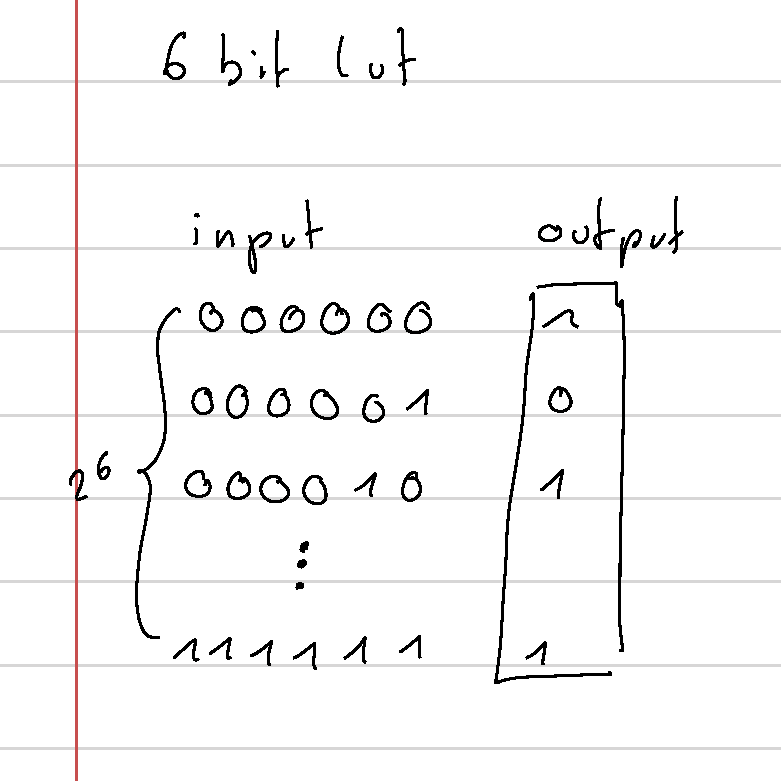
\includegraphics[width=.4\textwidth]{Figures/configuration_part1.pdf}
    \caption{LUT config vector}
    \label{fig:config_p1}
\end{figure}

To speed up the reconfiguration process, ZUMA configures blocks of \configvalue{config_width} LUTs in parallel, which are \(32\) by default. Each such block is internally called a stage.
For each stage ZUMA configures each line of the \(32\) LUTs step-by-step as shown in Figure~\ref{fig:config_p2}.
Therefore, every one of the \(32\) bits of each \hwport{config_data} value is used for a different LUT. ZUMA thus renames that input to \hwport{wr_data} and assigns the proper bit \hwport{wr_data[i]} as input to each LUT of a stage.
\begin{figure}[htbp]
    \centering
    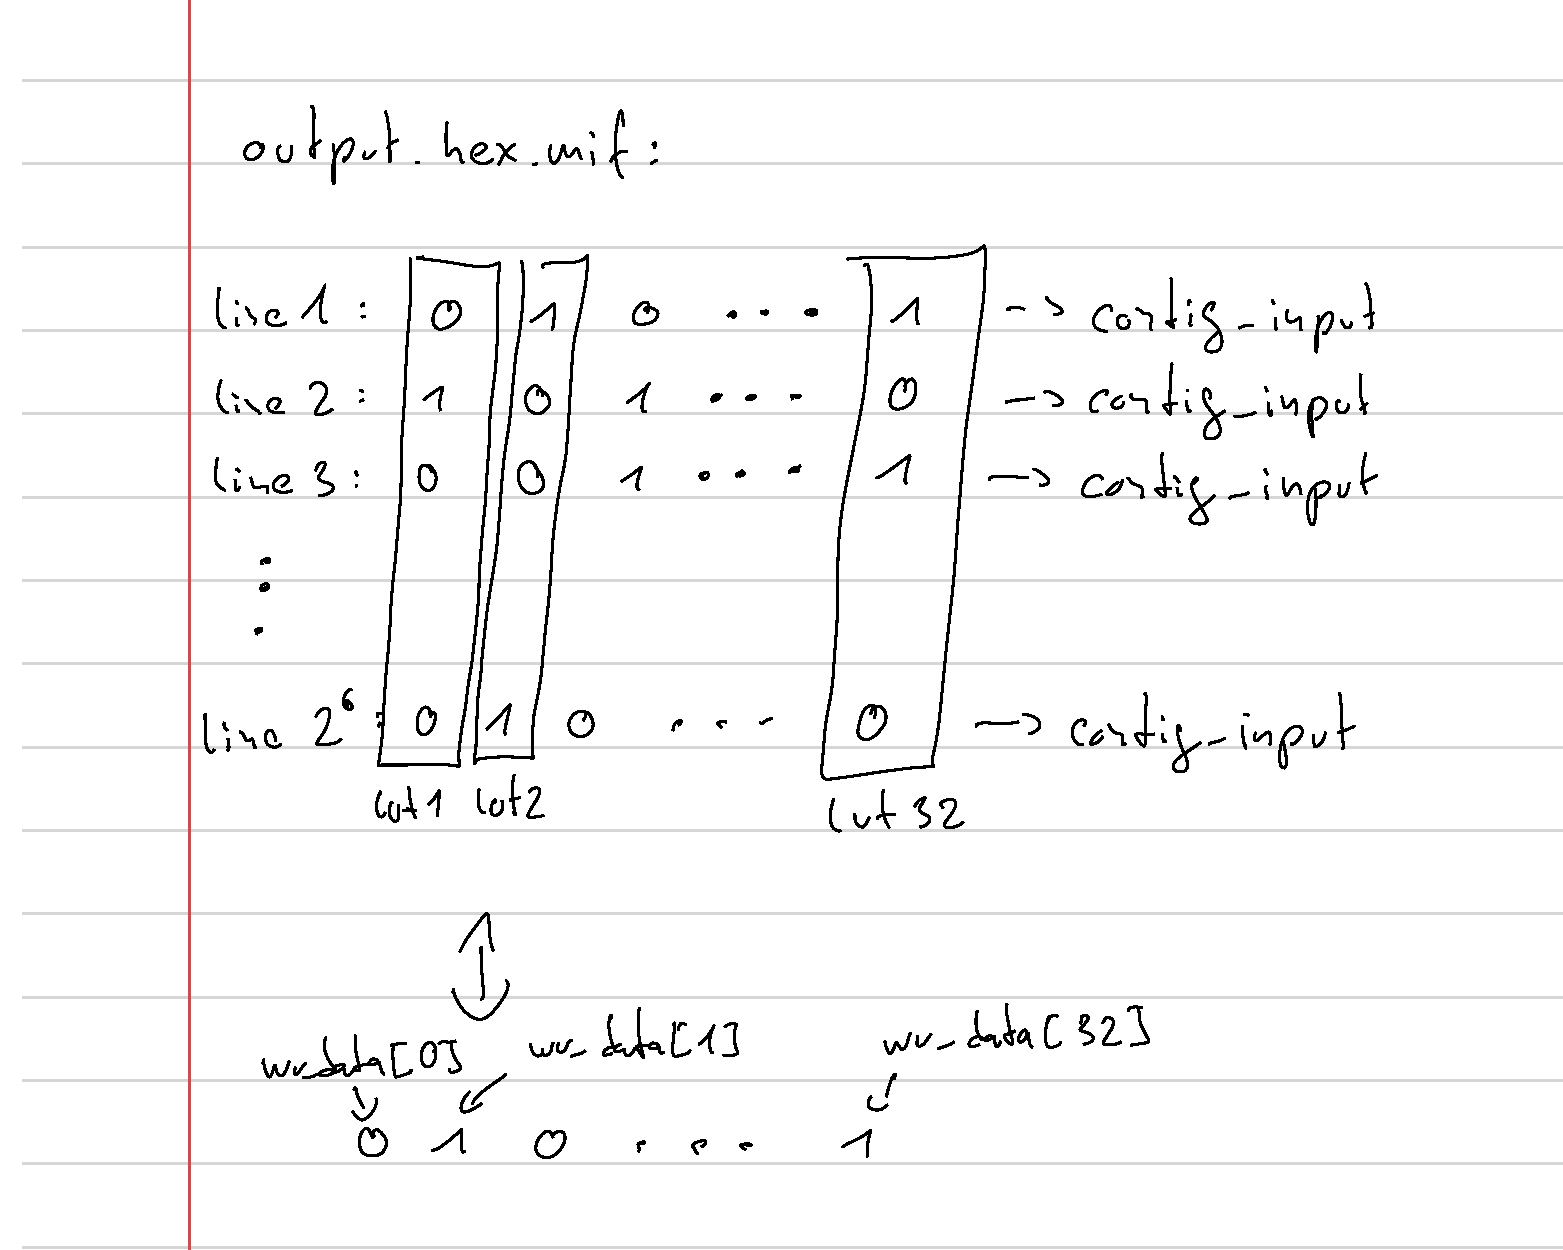
\includegraphics[width=.75\textwidth]{Figures/configuration_part2.pdf}
    \caption{configuration line per line}
    \label{fig:config_p2}
\end{figure}
To address only the LUTs of a single stage at a time during this configuration writing, ZUMA uses two address signals: \hwport{wr_addr} and \hwport{wren}.
These are assigned by the configuration controller module \module{config_controller_simple} as shown in Listing~\ref{lst:verilog_config_controller_simple.v}.

\begin{lstlisting}[style=Verilog,caption={{Excerpt from config\_controller\_simple.v.}}, float=htp, label={lst:verilog_config_controller_simple.v}]
    assign addr_out = addr_in[LUTSIZE-1:0];

    generate
        genvar stage;
        for(stage = 0; stage < STAGES; stage = stage+1) begin: stage_m
            assign wren[stage] = ((addr_in >> LUTSIZE) == stage) && wren_global;
        end
    endgenerate
\end{lstlisting}

\hwport{addr_out} is directly the last \hwport{LUTSIZE}-1 bits of the incoming \hwport{addr_in} signal of ZUMA, however, \hwport{wren} is a bit more special: For each stage number \emph{i}, only the \emph{i}-th bit \hwport{wren[i]} is $1$ while all the others are $0$.

To summarize:
The least significant \hwport{LUTSIZE} bits of the configuration address are thus used to walk the the lines of all \(32\) LUTs of a stage simultaneously, and the remaining upper bits are used to walk the stages.
The configuration process thus fully configures (up to) \(32\) LUTs in parallel and then switches to the next stage, until there are no unconfigured stages left.
Within each stage, the process configures all LUTs of that stage in parallel, line-by-line, until all \(2^{k_{host}}\) configuration bits are written.
Hence, the bitstream is also made up of blocks of \(2^{k_{host}}\) lines of \(32\)-bit values that directly correspond to this scheme.


\clearpage
\section{Comprehensive List of all Configuration Parameters} % (fold)
\label{sec:comprehensive_list_of_all_configuration_parameters}
%A list of all ZUMA configuration parameters with brief explanations:\\[1.5mm]
\renewcommand{\arraystretch}{1.2}%
\begin{xltabular}{\textwidth}{lcR}
    \caption{A list of all ZUMA configuration parameters with brief explanations.} \label{tab:all_configuration_parameters} \\

        \hline \multicolumn{1}{c}{\textbf{Parameter}} & \multicolumn{1}{c}{\textbf{Type}} & \multicolumn{1}{c}{\textbf{Description}} \\ \hline \hline
    \endfirsthead

        \multicolumn{3}{c}%
        {\tablename\ \thetable{} -- \textit{continued from previous page}} \\
        \hline \multicolumn{1}{c}{\textbf{Parameter}} & \multicolumn{1}{c}{\textbf{Type}} & \multicolumn{1}{c}{\textbf{Description}} \\ \hline \hline
    \endhead

        \hline \multicolumn{3}{r}{\textit{\small Continued on next page}} \\
    \endfoot

        \hline
    \endlastfoot


    % The table itself
    \multicolumn{3}{c}{\emph{General parameters}} \\
    \hline
    \configvalue{vprVersion} & Integer & Version of VPR included in installed VTR. Versions 6, 7, and 8 are supported (cp.~Section~\ref{sec:installation}). \\
    \configvalue{verifyOverlay} & Boolean & Enables an equivalence check of the generated overlay with the initial user circuit. Requires VPR 8 and Yosys (cp.~Section~\ref{sec:installation}). \\
    \configvalue{useClock} & Boolean & Needs to be correctly set for \configvalue{verifyOverlay} to inform it whether the virtual circuit uses a clock. \\
    \configvalue{packedOverlay} & Boolean & Enables an additional packed version of the overlay, ready for verification and building. \\


    \hline
    \multicolumn{3}{c}{\emph{Structural parameters}} \\
    \hline

    \multicolumn{3}{l}{\emph{Global structure}} \\
    \cline{1-2}
    \configvalue{X}             & Integer & Grid size in \emph{x} dimension \\
    \configvalue{Y}             & Integer & Grid size in \emph{y} dimension \\
    \configvalue{L}             & Integer & Length of the routing channels \\
    \configvalue{W}             & Integer & Number of tracks per routing channel \\
    \configvalue{orderedIO}     & Boolean & Whether or not to build large permutation MUXes around all IOs to fix their position in the \emph{fpga\_input\,/\,fpga\_output} arrays. \\

    \cline{1-2}
    \multicolumn{3}{l}{\emph{Local structure}} \\
    \cline{1-2}
    \configvalue{I}             & Integer & External cluster inputs (from connect block to IIB) \\
    \configvalue{N}             & Integer & LUTs per cluster \\
    \configvalue{K}             & Integer & LUT input width \\
    \configvalue{UseClos}       & Boolean & Whether the IIB should be Clos network-based (otherwise it is a fully connected crossbar). \\

    \cline{1-2}
    \multicolumn{3}{l}{\emph{Connect block}} \\
    \cline{1-2}
    \configvalue{fc_in}        & Float & From how many tracks of the connect block each of the \(I\) cluster inputs can be driven. \\
    \configvalue{fc_in_type}  & String & 'abs', or 'rel': Whether \configvalue{fc_in} is an absolute number or relative value. \\
    \configvalue{fc_out}       & Float & How many tracks of the connect block each of the \(N\) cluster outputs can drive.\\
    \configvalue{fc_out_type} & String & 'abs', or 'rel': Whether \configvalue{fc_out} is an absolute number or relative value. \\


    \hline
    \multicolumn{3}{c}{\emph{Configuration parameters}} \\
    \hline
    \configvalue{config_width}      & Integer & Width of the configuration port (in Bits). \\
    \configvalue{config_addr_width} & Integer & Width of the configuration addresses (in Bits). \\


    \hline
    \multicolumn{3}{c}{\emph{Parameters for hierarchical builds}} \\
    \hline

    \multicolumn{2}{l}{\emph{Module Separation}} & \vcenterothercols{Whether the resources of that type should be implemented hierarchically in the overlay fabric (\inlinepath{ZUMA_custom_generated.v}).} \\
    \cline{1-2}
    \configvalue{hierarchyNode} & Boolean & One module per ODG node. \\
    \configvalue{hierarchyInterConnect} & Boolean & One module per ???. \\
    \configvalue{hierarchyBle} & Boolean & One module per BLE. \\
    \configvalue{hierarchyCluster} & Boolean & One module per cluster\,/\,CLB. \\

    \cline{1-2}
    \multicolumn{2}{l}{\emph{Black box replacement}} & \vcenterothercols{Whether the resources of that type should be replaced by black boxes in the overlay fabric (\inlinepath{ZUMA_custom_generated.v}) -- useful later reorganization with tools such as RapidWright.} \\
    \cline{1-2}
    \configvalue{blackBox} & Boolean & Enable black box replacement in general. \\
    \configvalue{blackBoxBle} & Boolean & Replace BLEs with black boxes. \\
    \configvalue{blackBoxCluster} & Boolean & Replace clusters\,/\,CLBs with black boxes. \\
    \configvalue{blackBoxInterconnect} & Boolean & Replace ??? with black boxes. \\


    \hline
    \multicolumn{3}{c}{\emph{Timing Analysis and Optimization parameters}} \\
    \hline

    %\cline{1-2}
    \multicolumn{2}{l}{\emph{Timing Analysis}} & See Section~\ref{ssub:ZUMA_flow_details_timingdriven} \\
    \cline{1-2}
    \configvalue{sdf} & Boolean & Whether to activate the timing analysis. \\
    \configvalue{sdfFileName} & String & Path\,/\,Name of the first generated SDF file \inlinepath{Top_complete.sdf} (Vivado) or \inlinepath{Top_no_buffer.sdf} (ISE). \\
    \configvalue{sdfFlipflopFileName} & String & In case of an ISE flow: Path\,/\,Name of the second generated SDF file \inlinepath{Top_with_buffer.sdf}. \\
    \configvalue{timeScale}  & Float  & The time scale used in the provided SDF files as float, e.g., 1.0/1000000000000. \\
    \configvalue{timeFormat} & String & The time scale used in the provided SDF files as string, e.g., "ps". \\
    \configvalue{sdfUsedTool} & String & Indicator of the concrete SDF format. Implemented formats are the Xilinx flows ``ise'' and ``vivado''. \\
    \configvalue{sdfInterconnectCellType} & String & Vivado adds all interconnect to the top ZUMA cell, and hence we need its name to extract the delays. Typically should be \hwport{zuma_wrapper}. \\
    \configvalue{instancePrefix} & String & The path prefix that can be used to identify overlay components in the SDF files. For instance, the component \hwport{zuma_top/zuma_i} is translated to \hwport{zuma_top_zuma_i_} in the SDF file. For the standard TB wrapper, this would be \hwport{XUM/}. \\

    \cline{1-2}
    \multicolumn{2}{l}{\emph{Timing-driven placement \& routing}} & \vcenterothercols{} \\
    \cline{1-2}
    \configvalue{vprAnnotation} & Boolean & Whether VPR 8 should be used in timing-driven P\&R mode in a second run with the timing from the SDF file(s). Requires VPR 8 (cp.~Section~\ref{sec:installation}). \\
    \configvalue{setupTime} & Numberstring & Currently, setup times are not read from the SDF file, but have to be manually entered here. Example: ``4e-12''. \\
    \configvalue{holdTime}  & Numberstring & Currently, hold times are not read from the SDF file, but have to be manually entered here. Example: ``2.0e-9''. \\
%to have a finder control of the timing annotation:
    \configvalue{annotateOuterRouting} & Boolean & Whether the outer, global routing resources between CLBs should be annotated with their timing. \\
    \configvalue{annotateInnerRouting} & Boolean & Whether the inner, local routing resources inside CLBs should be  nnotated with their timing. \\

    \cline{1-2}
    \multicolumn{2}{l}{\emph{Timing analysis components}} & \vcenterothercols{Which parts of the virtual FPGA should contribute to the critical path and thus \(f_{max}\) calculation.} \\
    \cline{1-2}
    \configvalue{skipOrderedLayerTiming} & Boolean & If the delays of the ordering layer should be considered. These are only meaningful if \configvalue{orderedIO} is set to True. \\
    \configvalue{skipOuterRoutingTiming} & Boolean & Whether the outer, global routing resources between CLBs should be considered. \\
    \configvalue{skipInnerRoutingTiming} & Boolean & Whether the inner, local routing resources inside CLBs should be considered. \\


    \hline
    \multicolumn{3}{c}{\emph{Debugging and Visualization parameters}} \\
    \hline
    \configvalue{dumpNodeGraph} & Boolean & If set, the ODG and the technology-mapped ODG will be dumped into files in a readable format. \\
    \configvalue{graphviz} & Boolean & Makes \configvalue{dumpNodeGraph} also dump graphical versions of the ODGs -- \emph{WARNING}: Graphviz could freeze the build process if the graph is too big. \\
    \configvalue{dumpUnconfiguredNodes} & Boolean & If set, a list of unconfigured nodes with their Verilog names will be generated. \\

\end{xltabular}
% section comprehensive_list_of_all_configuration_parameters (end)

\addcontentsline{toc}{section}{References}
\bibliographystyle{unsrtnat}
\bibliography{ZUMA}

\end{document}
